\RequirePackage[l2tabu, orthodox]{nag}
\documentclass[version=last, pagesize, twoside=semi, DIV=calc, 12pt, a4paper, french, english, bibliography=totoc]{scrartcl}
%INSTALL

%avoids a warning
\usepackage[log-declarations=false]{xparse}
\usepackage{fontspec} %font selecting commands
\usepackage{xunicode}
\usepackage{ucharclasses}
%warn about missing characters
\tracinglostchars=2

%REDAC
\usepackage{booktabs}
\usepackage{calc}
\usepackage{tabularx}

\usepackage{etoolbox} %for addtocmd, newtoggle commands
\newtoggle{LCpres}
\togglefalse{LCpres}

\usepackage{mathtools} %load this before babel!
	\mathtoolsset{showonlyrefs,showmanualtags}

%\usepackage[french, english]{babel}%options should probably be on the document level
\usepackage{babel}
%suppresses the warning about frenchb not modifying the captions (“—” to “:” in “Figure 1 – Legend”).
%	\frenchbsetup{AutoSpacePunctuation=false,SuppressWarning=true}% test with false?
	\frenchbsetup{AutoSpacePunctuation=false,SuppressWarning=false}

%\usepackage[super]{nth}%better use fmtcount! (loaded by datetime anyway; see below about pbl with warnings and package silence)
\usepackage{listings} %typeset source code listings
	\lstset{language=XML,tabsize=2,captionpos=b,basicstyle=\NoAutoSpacing}%NoAutoSpacing avoids space before colon or ?}%,literate={"}{{\tt"}}1, keywordstyle=\fontspec{Latin Modern Mono Light}\textbf, emph={String, PreparedStatement}, emphstyle=\fontspec{Latin Modern Mono Light}\textbf, language=Java, basicstyle=\small\NoAutoSpacing\ttfamily, aboveskip=0pt, belowskip=0pt, showstringspaces=false
\usepackage[nolist,smaller,printonlyused]{acronym}%,smaller option produces warnings from relsize in some cases, it seems.% Note silence and acronym and hyperref make (xe)latex crash when ac used in section (http://tex.stackexchange.com/questions/103483/strange-packages-interaction-acronyms-silence-hyperref), rather use \section{\texorpdfstring{\acs{UE}}{UE}}.
\usepackage{fmtcount}
\usepackage[nodayofweek]{datetime}%must be loaded after the babel package. However, loading it after {nth} generates a warning from fmtcount about ordinal being already defined. Better load it before nth? (then we can remove the silence package which creates possible crashes, see above.) Or remove nth?
%\usepackage{xspace}%do we need this?
\nottoggle{LCpres}{
	\usepackage[textsize=small]{todonotes}
}{
}
\iftoggle{LCpres}{
	%remove pdfusetitle (implied by beamer)
	\usepackage{hyperref}
}{
% option pdfusetitle must be introduced here, not in hypersetup.
	\usepackage[pdfusetitle]{hyperref}
}
%breaklinks makes links on multiple lines into different PDF links to the same target.
%colorlinks (false): Colors the text of links and anchors. The colors chosen depend on the the type of link. In spite of colored boxes, the colored text remains when printing.
%linkcolor=black: this leaves other links in colors, e.g. refs in green, don't print well.
%pdfborder (0 0 1, set to 0 0 0 if colorlinks): width of PDF link border
%hidelinks
\hypersetup{breaklinks, bookmarksopen}
%add hyperfigures=true in hypersetup (already defined in article mode)
\iftoggle{LCpres}{
	\hypersetup{hyperfigures}
}{
}

%in Beamer, sets url colored links but does not change the rest of the colors (http://tex.stackexchange.com/questions/13423/how-to-change-the-color-of-href-links-for-real)
%\hypersetup{breaklinks,bookmarksopen,colorlinks=true,urlcolor=blue,linkcolor=,hyperfigures=true}
% hyperref doc says: Package bookmark replaces hyperref’s bookmark organization by a new algorithm (...) Therefore I recommend using this package.
\usepackage{bookmark}

% center floats by default, but do not use with float
% \usepackage{floatrow}
% \makeatletter
% \g@addto@macro\@floatboxreset\centering
% \makeatother
\nottoggle{LCpres}{
	\usepackage{enumitem} %follow enumerate by a string saying how to display enumeration
}{
}
\usepackage{ragged2e} %new com­mands \Cen­ter­ing, \RaggedLeft, and \RaggedRight and new en­vi­ron­ments Cen­ter, FlushLeft, and FlushRight, which set ragged text and are eas­ily con­fig­urable to al­low hy­phen­ation (the cor­re­spond­ing com­mands in LaTeX, all of whose names are lower-case, pre­vent hy­phen­ation al­to­gether). 
\usepackage{siunitx} %[expproduct=tighttimes, decimalsymbol=comma] ou (plus récent ?) [round-mode=figures, round-precision=2, scientific-notation = engineering]
\sisetup{detect-all, locale = FR, strict}% to detect e.g. when in math mode (use a math font) - check whether this makes sense with strict
\usepackage{braket} %for \Set
\usepackage{natbib}
\usepackage{bibentry}
%\usepackage{doi}

\usepackage{amsmath,amsthm}
% \usepackage{amsfonts} %not required?
% \usepackage{dsfont} %for what?
%unicode-math overwrites the following commands from the mathtools package: \dblcolon, \coloneqq, \Coloneqq, \eqqcolon. Using the other colon-like commands from mathtools will lead to inconsistencies. Plus, Using \overbracket and \underbracke from mathtools package. Use \Uoverbracket and \Uunderbracke for original unicode-math definition.
%use exclusively \mathbf and choose math bold style below.
\usepackage[warnings-off={mathtools-colon, mathtools-overbracket}, bold-style=ISO]{unicode-math}

%\defaultfontfeatures{
%	Fractions=On,
%	Mapping=tex-text% to turn "--" into dashes, useful for bibtex%%
%}
%\defaultfontfeatures[\rmfamily, \sffamily]{
%\defaultfontfeatures[\rmfamily]{
%	Fractions=On,
%	Mapping=% to leave " alone (disable the default mapping tex-text; requires loading the font afterwards?)
%}
%\newfontfamily\xitsfamily{XITS}
\newfontfamily\mulifamily{Muli}
\newfontfamily\texgyretermesfamily{TeX Gyre Termes}
\newfontfamily\texgyreherosfamily{TeX Gyre Heros}
\newfontfamily\lmfamily{Latin Modern Roman}
\iftoggle{LCpres}{
	\setmainfont{Latin Modern Roman}
	\setsansfont{Latin Modern Sans}
	\setmonofont{Latin Modern Mono}
}{
	\setmainfont{TeX Gyre Termes}
%	\setsansfont{TeX Gyre Heros}
	\setsansfont{Muli}
	\setmonofont{TeX Gyre Cursor}
}
\defaultfontfeatures{}%disable default font features to avoid warnings with math fonts.
%\setmathfont{XITS Math}
%\setmathfont[range={\mathcal,\mathbfcal},StylisticSet=1]{XITS Math}
%to make \boldmath $\cdot$ work (otherwise: “Missing character: There is no ⋅ in font XITS Math Bold/OT:script=math;language =DFLT;!”). Alternative: \setmathfont[BoldFont=XITS Math]{XITS Math}
%\setmathfont[range={"22C5},version=bold]{XITS Math}
%silently delays restoring normal font when using e.g. “≠)” or “≠ other word”.
%\setTransitionTo{Arrows}{\xitsfamily}
%\setTransitionTo{MathematicalOperators}{\xitsfamily}
%this solution explicitly fails on “≠)” and works for “≠ other word.”
%\setTransitionsFor{MathematicalOperators}{\begingroup\xitsfamily}{\endgroup}
%\setTransitionsFor{Arrows}{\begingroup\xitsfamily}{\endgroup}
%texgyretermes does not have ✓, XITS does.
%\setTransitionsFor{Dingbats}{\begingroup\xitsfamily}{\endgroup}
%this also works, but it is more complex
%\def\ResetTransitionTo#1{%
%  \XeTeXinterchartoks 255 \csname#1Class\endcsname{\relax}}
%\setTransitionsFor{MathematicalOperators}
%  {\begingroup\ResetTransitionTo{MathematicalOperators}\xitsfamily}
%  {\endgroup}

\usepackage{environ}%for xdescwd command
\usepackage{cleveref}% cleveref should go "laster" than hyperref
%GRAPHICS
\usepackage{pgf}
\usepackage{pgfplots}
	\usetikzlibrary{babel, matrix, fit, plotmarks, calc, trees, shapes.geometric, positioning, plothandlers, arrows, shapes.multipart}
\pgfplotsset{compat=1.11}
\usepackage{graphicx}

\graphicspath{{graphics/},{graphics-dm/}}
\DeclareGraphicsExtensions{.pdf}
\LetLtxMacro\SavedIncludeGraphics\includegraphics
\AtBeginDocument{
	\def\includegraphics#1#{% #1 catches optional stuff (star/opt. arg.)
		\IncludeGraphicsAux{#1}%
	}%
}
\newcommand*{\IncludeGraphicsAux}[2]{%
	\XeTeXLinkBox{%
		\SavedIncludeGraphics#1{#2}%
	}%
}%

%HACKING
\usepackage{printlen}
\uselengthunit{mm}
% 	\newlength{\templ}% or LenTemp?
% 	\setlength{\templ}{6 pt}
% 	\printlength{\templ}
\usepackage{scrhack}% load at end. Corrects a bug in float package, which is outdated but might be used by other packages
\usepackage{xltxtra} %somebody said that this is loaded by fontspec, but does not seem correct: if not loaded explicitly, does not appear in the log and \showhyphens is not corrected.

%Beamer-specific
%do not remove babel, which beamer uses (beamer uses the \translate command for the appendix); but french can be removed.
\iftoggle{LCpres}{
	\usepackage{appendixnumberbeamer}
	\setbeamertemplate{navigation symbols}{} 
	\usepackage{preamble/beamerthemeParisFrance}
	\usefonttheme{professionalfonts}
	\setcounter{tocdepth}{10}
	%From: http://tex.stackexchange.com/questions/168057/beamer-with-xelatex-on-texlive2013-enumerate-numbers-in-black
%I don’t think it’s useful to submit this as a bug: nothing has been solved since March, 2015. See: https://bitbucket.org/rivanvx/beamer/issues?status=resolved.

\setbeamertemplate{enumerate item}
{
  \begin{pgfpicture}{-1ex}{-0.65ex}{1ex}{1ex}
    \usebeamercolor[fg]{item projected}
    {\pgftransformscale{1.75}\pgftext{\normalsize\pgfuseshading{bigsphere}}}
    {\pgftransformshift{\pgfpoint{0pt}{0.5pt}}
      \pgftext{\usebeamercolor[fg]{item projected}\usebeamerfont*{item projected}\insertenumlabel}}
  \end{pgfpicture}%
}

\setbeamertemplate{enumerate subitem}
{
  \begin{pgfpicture}{-1ex}{-0.55ex}{1ex}{1ex}
    \usebeamercolor[fg]{subitem projected}
    {\pgftransformscale{1.4}\pgftext{\normalsize\pgfuseshading{bigsphere}}}
    \pgftext{%
      \usebeamercolor[fg]{subitem projected}%
      \usebeamerfont*{subitem projected}%
      \insertsubenumlabel}
  \end{pgfpicture}%
}

\setbeamertemplate{enumerate subsubitem}
{
  \begin{pgfpicture}{-1ex}{-0.55ex}{1ex}{1ex}
    \usebeamercolor[fg]{subsubitem projected}
    {\pgftransformscale{1.4}\pgftext{\normalsize\pgfuseshading{bigsphere}}}
    \pgftext{%
      \usebeamercolor[fg]{subsubitem projected}%
      \usebeamerfont*{subitem projected}%
      \insertsubsubenumlabel}
  \end{pgfpicture}%
}


}{
}
% \newcommand{\citep}{\cite}%Better: leave natbib.
% \setbeamersize{text margin left=0.1cm, text margin right=0.1cm} 
% \usetheme{BrusselsBelgium}%no, replace with paris
%\usetheme{ParisFrance}, no, usepackage better!
% Tex Gyre takes too much space, replace with Latin Modern Roman / Sans / Mono.
% Difference when loading explicitly Latin Modern Sans (compared to not using \setsansfont at all):
% the font LMSans17-Regular appears in the document;
% the title of the slides appears differently;
% it does not say (in the log file):
% > LaTeX Font Info:    Font shape `EU1/lmss/m/it' in size <10.95> not available
% > (Font)              Font shape `EU1/lmss/m/sl' tried instead on input line 85.
% > LaTeX Font Info:    Try loading font information for EU1+lmtt on input line 85.

%tikzposter-specific
%remove \usepackage{ragged2e}: causes 1=1 to be printed in the middle of the poster. (Anyway prints a warning about those characters being missing.)
%put [french, english] options next to \usepackage{babel} to avoid warning of 

\newcommand{\R}{ℝ}
\newcommand{\N}{ℕ}
\newcommand{\Z}{ℤ}
\newcommand{\card}[1]{\lvert{#1}\rvert}
\newcommand{\powerset}[1]{\mathscr{P}(#1)}%\mathscr rather than \mathcal: scr is rounder than cal (at least in XITS Math).
\newcommand{\suchthat}{\;\ifnum\currentgrouptype=16 \middle\fi|\;}
%\newcommand{\Rplus}{\reels^+\xspace}

\AtBeginDocument{%
	\renewcommand{\epsilon}{\varepsilon}
% we want straight form of \phi for mathematics, as recommended in UTR #25: Unicode support for mathematics.
%	\renewcommand{\phi}{\varphi}
}

% with amssymb, but I don’t want to use amssymb just for that.
% \newcommand{\restr}[2]{{#1}_{\restriction #2}}
%\newcommand{\restr}[2]{{#1\upharpoonright}_{#2}}
\newcommand{\restr}[2]{{#1|}_{#2}}%sometimes typed out incorrectly within \set.
%\newcommand{\restr}[2]{{#1}_{\vert #2}}%\vert errors when used within \Set and is typed out incorrectly within \set.
\DeclareMathOperator*{\argmax}{arg\,max}
\DeclareMathOperator*{\argmin}{arg\,min}


%Voting and MCDA
\newcommand{\allalts}{\mathscr{A}}
\newcommand{\alts}{A}
\newcommand{\allF}{\mathcal{F}}
\newcommand{\cat}[1]{C_{#1}}

%Voting
\newcommand{\feasalts}{F}
\newcommand{\allvoters}{\mathscr{N}}
\newcommand{\voters}{N}
\newcommand{\allsystems}{\mathcal{G}}
\newcommand{\prof}{\mathbf{R}}
\newcommand{\allprofs}{\mathbfcal{R}}
\newcommand{\linors}{\mathcal{L}(\alts)}

\newcommand{\pbasic}[1]{\prof^{#1}_\epsilon}
\newcommand{\pelem}[1]{\prof^{#1}_e}
\newcommand{\pcycl}[1]{\prof^{#1}_c}
\newcommand{\pcycllong}[1]{\prof^{#1}_{cl}}
\newcommand{\pinv}[1]{\overline{\prof_{#1}}}
\newcommand{\dmap}{{\xitsfamily δ}}
%powerset without zero
\newcommand{\powersetz}[1]{\mathcal{P}_\emptyset(#1)}

%logic atom
%⟼ (long)
\DeclareDocumentCommand{\lato}{ O{\prof} O{\alts} }{[#1 \!⟼\! #2]}
%logic atom in
%↝, \stackrel{\in}{\mapsto}, ➲, ⥹
\newcommand{\tightoverset}[2]{%
  \mathop{#2}\limits^{\vbox to -.5ex{\kern-0.9ex\hbox{$#1$}\vss}}}
\DeclareDocumentCommand{\latoin}{ O{\prof} O{\alpha} }{[#1 \tightoverset{\in}{⟼} #2]}
\newcommand{\alllang}{\mathcal{L}}
\newcommand{\ltru}{\texttt{T}}
\newcommand{\lfal}{\texttt{F}}
\newcommand{\laxiom}[1]{{\texgyreherosfamily{\textsc{#1}}}}

%ARG TH
\newcommand{\AF}{\mathcal{AF}}
\newcommand{\labelling}{\mathcal{L}}
\newcommand{\labin}{\textbf{in}\xspace}
\newcommand{\labout}{\textbf{out}}
\newcommand{\labund}{\textbf{undec}\xspace}
\newcommand{\nonemptyor}[2]{\ifthenelse{\equal{#1}{}}{#2}{#1}}
\newcommand{\gextlab}[2][]{
	\labelling{\mathcal{GE}}_{(#2, \nonemptyor{#1}{\ibeatsr{#2}})}
}
\newcommand{\allargs}{A^*}
\newcommand{\args}{A}
\newcommand{\ar}{a}
\newcommand{\ext}{\mathcal{E}}

%MCDA+Arg
\newcommand{\dm}{d}
\newcommand{\ileadsto}{\rightcurvedarrow}
\newcommand{\mleadsto}[1][\eta]{\rightcurvedarrow_{#1}}
\newcommand{\ibeats}{\vartriangleright}
\newcommand{\mbeats}[1][\eta]{\vartriangleright_{#1}}

%MISC
\newcommand{\lequiv}{\Vvdash}
\newcommand{\weightst}{W^{\,t}}

%MCDA classical
\newcommand{\crits}{\mathcal{J}}

%Sorting
\newcommand{\cats}{\mathcal{C}}
\newcommand{\catssubsets}{2^\cats}
\newcommand{\catgg}{\vartriangleright}
\newcommand{\catll}{\vartriangleleft}
\newcommand{\catleq}{\trianglelefteq}
\newcommand{\catgeq}{\trianglerighteq}
\newcommand{\alttoc}[2][x]{(#1 \xrightarrow{} #2)}
\newcommand{\alttocat}[3]{(#2 \xrightarrow{#1} #3)}
\newcommand{\alttoI}{(x \xrightarrow{} \left[\underline{C_x}, \overline{C_x}\right])}
\newcommand{\alttocatdm}[3][t]{\left(#2 \thinspace \raisebox{-3pt}{$\xrightarrow{#1}$}\thinspace #3\right)}
\newcommand{\alttocatatleast}[2]{\left(#1 \thinspace \raisebox{-3pt}{$\xrightarrow[]{≥}$}\thinspace #2\right)}
\newcommand{\alttocatatmost}[2]{\left(#1 \thinspace \raisebox{-3pt}{$\xrightarrow[]{≤}$}\thinspace #2\right)}

\definecolor{darkgreen}{rgb}{0,0.6,0}
\newcommand{\commentOC}[1]{{\small\color{blue}{\selectlanguage{french}$\big[$OC: #1$\big]$}}}
%\newcommand{\commentOC}[1]{{\selectlanguage{french}{\todo{OC : #1}}}}
%Or: \todo[color=green!40]
\newcommand{\innote}[1]{{\scriptsize{#1}}}

%this probably requires outdated float package, see doc KomaScript for an alternative.
% \newfloat{program}{t}{lop}
% \floatname{program}{PM}

%definition, theorem, lemma, example environments, qed trickery are only needed in article mode (not Beamer)
\nottoggle{LCpres}{
%style is plain by default (italic text)
	\newtheorem{definition}{Definition}
	\newtheorem{theorem}{Theorem}
%no italic: expected.
%http://tex.stackexchange.com/questions/144653/italicizing-of-amsthm-package
	\newtheorem{lemma}{Lemma}
%\crefname{axiom}{axiom}{axioms}%might be needed for workaround bug in cref when defining new theorems?

%\ifdefined\theorem\else
%\newtheorem{theorem}{\iflanguage{english}{Theorem}{Théorème}}
%\fi

\theoremstyle{remark}
	\newtheorem{examplex}{Example}
	\newtheorem{remarkx}{Remark}

%trickery allowing use of \qedhere and the like.
\newenvironment{example}{
	\pushQED{\qed}\renewcommand{\qedsymbol}{$\triangle$}\examplex
}{
	\popQED\endexamplex
}
\newenvironment{remark}{
	\pushQED{\qed}\renewcommand{\qedsymbol}{$\triangle$}\remarkx
}{
	\popQED\endremarkx
}
}{
}
\crefname{examplex}{example}{examples}% I wonder why this is unnecessary in case of singular

%which line breaks are chosen: accept worse lines, therefore reducing risk of overfull lines. Default = 200
\tolerance=2000
%accept overfull hbox up to...
\hfuzz=2cm
%reduces verbosity about the bad line breaks
\hbadness 5000
%sloppy sets tolerance to 9999
\apptocmd{\sloppy}{\hbadness 10000\relax}{}{}

\bibliographystyle{abbrvnat}
%\bibliographystyle{plainnat}
%or \bibliographystyle{apalike} for presentations?

%doi package uses old-style dx.doi url, see 3.8 DOI system Proxy Server technical details, “Users may resolve DOI names that are structured to use the DOI system Proxy Server (http://doi.org (preferred) or http://dx.doi.org).”, https://www.doi.org/doi_handbook/3_Resolution.html
\makeatletter
\patchcmd{\@doi}{dx.doi.org}{doi.org}{}{}
\makeatother

% WRITING
%\newcommand{\ie}{i.e.\@\xspace}%to try
%\newcommand{\eg}{e.g.\@\xspace}
%\newcommand{\etal}{et al.\@\xspace}
\newcommand{\ie}{i.e.\ }
\newcommand{\eg}{e.g.\ }
\newcommand{\mkkOK}{\checkmark}%\color{green}{\checkmark}
\newcommand{\mkkREQ}{\ding{53}}%requires pifont?%\color{green}{\checkmark}
\newcommand{\mkkNO}{}%\text{\color{red}{\textsf{X}}}

\newlength{\xdescwd}
\makeatletter
\NewEnviron{xdesc}{%
  \setbox0=\vbox{\hbadness=\@M \global\xdescwd=0pt
    \def\item[##1]{%
      \settowidth\@tempdima{\textbf{##1}:}%
      \ifdim\@tempdima>\xdescwd \global\xdescwd=\@tempdima\fi}
  \BODY}
  \begin{description}[leftmargin=\dimexpr\xdescwd+.5em\relax,
    labelindent=0pt,labelsep=.5em,
    labelwidth=\xdescwd,align=left]\BODY\end{description}}
\makeatother

\makeatletter
\newcommand{\boldor}[2]{%
	\ifnum\strcmp{\f@series}{bx}=\z@
		#1%
	\else
		#2%
	\fi
}
\newcommand{\textstyleElProm}[1]{\boldor{\MakeUppercase{#1}}{\textsc{#1}}}
\makeatother
\newcommand{\electre}{\textstyleElProm{Électre}\xspace}
\newcommand{\electreIv}{\textstyleElProm{Électre Iv}\xspace}
\newcommand{\electreIV}{\textstyleElProm{Électre IV}\xspace}
\newcommand{\electreIII}{\textstyleElProm{Électre III}\xspace}
\newcommand{\electreTRI}{\textstyleElProm{Électre Tri}\xspace}
% \newcommand{\utadis}{\texorpdfstring{\textstyleElProm{utadis}\xspace}{UTADIS}}
% \newcommand{\utadisI}{\texorpdfstring{\textstyleElProm{utadis i}\xspace}{UTADIS I}}

%TODO
% \newcommand{\textstyleElProm}[1]{{\rmfamily\textsc{#1}}} 


%const
\newcommand{\tikzboxit}{\path node[draw, overlay, inner sep=0.6mm, fit=(boxed), rectangle] {};}%

\newlength{\GraphsNodeSep}
\setlength{\GraphsNodeSep}{7mm}

% MCDA Drawing Sorting
\newlength{\MCDSCatHeight}
\setlength{\MCDSCatHeight}{6mm}
\newlength{\MCDSAltHeight}
\setlength{\MCDSAltHeight}{4mm}
%separation between two vertical alts
\newlength{\MCDSAltSep}
\setlength{\MCDSAltSep}{2mm}
\newlength{\MCDSCatWidth}
\setlength{\MCDSCatWidth}{3cm}
\newlength{\MCDSAltWidth}
\setlength{\MCDSAltWidth}{2.5cm}
\newlength{\MCDSEvalRowHeight}
\setlength{\MCDSEvalRowHeight}{6mm}
\newlength{\MCDSAltsToCatsSep}
\setlength{\MCDSAltsToCatsSep}{1.5cm}
\newcounter{MCDSNbAlts}
\newcounter{MCDSNbCats}
\newlength{\MCDSArrowDownOffset}
\setlength{\MCDSArrowDownOffset}{0mm}

\tikzset{/Graphs/dot/.style={
	shape=circle, fill=black, inner sep=0, minimum size=1mm
}}
\tikzset{/MC/D/S/alt/.style={
	shape=rectangle, draw=black, inner sep=0, minimum height=\MCDSAltHeight, minimum width=\MCDSAltWidth
}}
\tikzset{MC/D/S/pref/.style={
	shape=ellipse, draw=gray, thick
}}
\tikzset{/MC/D/S/cat/.style={
	shape=rectangle, draw=black, inner sep=0, minimum height=\MCDSCatHeight, minimum width=\MCDSCatWidth
}}
\tikzset{/MC/D/S/evals matrix/.style={
	matrix, row sep=-\pgflinewidth, column sep=-\pgflinewidth, nodes={shape=rectangle, draw=black, inner sep=0mm, text depth=0.5ex, text height=1em, minimum height=\MCDSEvalRowHeight, minimum width=12mm}, nodes in empty cells, matrix of nodes, inner sep=0mm, outer sep=0mm, row 1/.style={nodes={draw=none, minimum height=0em, text height=, inner ysep=1mm}}
}}

\newlength{\GitCommitSep}
\setlength{\GitCommitSep}{13mm}

\tikzset{/Git/commit/.style={
	shape=rectangle, draw, minimum width=4em, minimum height=0.6cm
}}
\tikzset{/Git/branch/.style={
	shape=ellipse, draw, red
}}
\tikzset{/Git/head/.style={
	shape=ellipse, draw, fill=yellow
}}

\tikzset{profile matrix/.style={
	matrix of math nodes, column sep=3mm, row sep=2mm, nodes={inner sep=0.5mm, anchor=base}
}}
\tikzset{rank-profile matrix/.style={
	matrix of math nodes, column sep=3mm, row sep=2mm, nodes={anchor=base}, column 1/.style={nodes={inner sep=0.5mm}}, row 1/.style={nodes={inner sep=0.5mm}}
}}
\tikzset{rank-vector/.style={
	draw, rectangle, inner sep=0, outer sep=1mm
}}
\tikzset{isolated rank-vector/.style={
	draw, matrix of math nodes, column sep=3mm, inner sep=0, matrix anchor=base, nodes={anchor=base, inner sep=.33em}, ampersand replacement=\&
}}

% GUI
\tikzset{/GUI/button/.style={
	rectangle, very thick, rounded corners, draw=black, fill=black!40%, top color=black!70, bottom color=white
}}

% Logger objects
\tikzset{/logger/main/.style={
	shape=rectangle, draw=black, inner sep=1ex, minimum height=7mm
}}
\tikzset{/logger/helper/.style={
	shape=rectangle, draw=black, dashed, minimum height=7mm
}}
\tikzset{/logger/helper line/.style={
	<->, draw, dotted
}}

% Beliefs
\tikzset{/Beliefs/D/S/attacker/.style={
	shape=rectangle, draw, minimum size=8mm
}}
\tikzset{/Beliefs/D/S/supporter/.style={
	shape=circle, draw
}}

\newcommand{\tikzmark}[1]{%
	\tikz[overlay, remember picture, baseline=(#1.base)] \node (#1) {};%
}


\begin{acronym}
\acro{AMCD}{Aide Multicritère à la Décision}
\acro{ASA}{Argument Strength Assessment}
\acro{DA}{Decision Analysis}
\acro{DM}{Decision Maker}
\acro{DPr}{Deliberated Preferences}
\acro{DRSA}{Dominance-based Rough Set Approach}
\acro{DSS}{Decision Support Systems}
\acrodefplural{DSS}{Decision Support Systems}
% \newacroplural{DSS}[DSSes]{Decision Support Systems}
\acro{EJOR}{European Journal of Operational Research}
\acro{LNCS}{Lecture Notes in Computer Science}
\acro{MCDA}{Multicriteria Decision Aid}
\acro{MIP}{Mixed Integer Program}
\acro{NCSM}{Non Compensatory Sorting Model}
\acro{PL}{Programme Linéaire}
\acro{PLNE}{Programme Linéaire en Nombres Entiers}
\acro{PM}{Programme Mathématique}
\acro{MP}{Mathematical Program}
\acro{MIP}{Mixed Integer Program}
% \newacroplural{PM}{Programmes Mathématiques}
%acrodefplural since version 1.35, my debian has \ProvidesPackage{acronym}[2009/01/25, v1.34, Support for acronyms (Tobias Oetiker)]
\acrodefplural{PM}{Programmes Mathématiques}
\acro{PMML}{Predictive Model Markup Language}
\acro{RESS}{Reliability Engineering \& System Safety}
\acro{SMAA}{Stochastic Multicriteria Acceptability Analysis}
\acro{URPDM}{Uncertainty and Robustness in Planning and Decision Making}
\acro{XML}{Extensible Markup Language}
\end{acronym}

\usepackage[official,right]{eurosym}
\nobibliography{lamsade}
%package doi does not work with bibentry. Need to replace it with this command, to protect doi's with \url.
\newcommand*{\doi}[1]{\href{http://doi.org/#1}{\url{doi: #1}}}
\usepackage{geometry}
\geometry{margin=2.8cm}
\renewcommand{\cite}{\citep}

\begin{document}
\title{Research report HCERES 2017}
\author{LAMSADE}
\hypersetup{
	pdfsubject={Research report}
}

\begin{titlepage}
	\centering
	\vspace*{\baselineskip} % White space at the top of the page
	{
		\LARGE 
		CNRS
		
		PSL Research University
		
		Université Paris-Dauphine
	
		\vspace{7em}
		
		\rule{15em}{1.6pt}
		\vspace{0.5\baselineskip}
	
		Laboratoire \textsc{Lamsade}
		
		UMR 7243
		\vspace{-0.5\baselineskip}

		\rule{15em}{1.6pt}
	
		\vspace{7em}
	
		Scientific Report and Project
		
		2012 -- 2017
		
		\vfill
		
	}
	\url{http://www.lamsade.dauphine.fr}
	
\end{titlepage} 

\pagestyle{empty}

\vspace*{5cm}
{\flushright%
	à Eric Jacquet-Lagrèze\\
	1947 -- 2017\par
}
\newpage

\renewcommand{\baselinestretch}{0.97}\normalsize
\tableofcontents
\renewcommand{\baselinestretch}{1.0}\normalsize
\newpage
\null
\newpage
\pagestyle{plain}
\setcounter{page}{1}

\definecolor{redh}{RGB}{255,0,102}

{%
	\centering%
		\colorbox{redh}{%
			\begin{minipage}{12.75cm}
%				\rule{\columnwidth}{1ex}
				\begin{center}
					\color{white}
					\Large \sffamily%
						\vspace{1em}
						Group D\par
						Evaluation campaign 2017 – 2018\par
						\vspace{1em}
						Research unit\par
						\vspace{1em}
						Application
				\end{center}
			\end{minipage}%
		}
	\par
}

\vspace{2em} 
\noindent\textcolor{redh}{\rule{\columnwidth}{1pt}}\par

\noindent
\textbf{Unit name}: Laboratoire d'Analyse et Modélisation de Systèmes d'Aide à la Décision \\
\textbf{Acronym}: LAMSADE, UMR 7243

\vspace{1em}

\noindent
\textbf{Director's name (current contract)}: Alexis Tsoukiàs \\
\textbf{Director's name (next contract)}: Daniela Grigori (pending approval)\\
\noindent\textcolor{redh}{\rule{\columnwidth}{1pt}}\par

\vspace{1em}

\noindent
Application type: 

\noindent\textcolor{redh}{\rule{\columnwidth}{1pt}}\par
Renewal (without important modification) \\%☑
\noindent\textcolor{redh}{\rule{\columnwidth}{1pt}}\par

\vspace{1em}

\noindent
List of supervising institutions and bodies of the research unit:

\noindent\textcolor{redh}{\rule{\columnwidth}{1pt}}\par
\begin{tabular}{ll}
%	\toprule
		Current contract & Next contract \\
%	\midrule
		Université Paris Dauphine & Université Paris Dauphine \\
		CNRS & CNRS \\
%	\bottomrule
\end{tabular}\\
\noindent\textcolor{redh}{\rule{\columnwidth}{1pt}}\par 

\vspace{1em}

\noindent
Inter-disciplinary evaluation for the research unit: 

\noindent\textcolor{redh}{\rule{\columnwidth}{1pt}}\par
Yes \\
\noindent\textcolor{redh}{\rule{\columnwidth}{1pt}}\par

\newpage
\pagestyle{empty}
\null
\newpage
\pagestyle{plain}

% !TeX root = rapport.tex
\section{Presentation}\label{presentation}

The LAMSADE is an historical research unit (established in 1974) originally created around the domain of Management Science and Operational Research, and then having evolved into Computer Science while keeping a very specific identity: Decision Sciences and Technologies. In this long history the unit has kept clear three distinctive features of its identity: \\
 - an original vision of Decision Sciences and Technologies, including an interdisciplinary perspective; \\
 - an international leadership through the establishment and the conduction of ``research communities''; \\
 - a wise blend between foundational and applied research, the field of decision sciences and technologies being specifically characterised by the necessity to keep the frontiers between these two fields widely open.

The research conducted within the LAMSADE aims at approaching the problem of improving both decision making and decision support (aiding to decision making) taking into account the axiomatic, algorithmic and pragmatic dimensions of these topics. The axiomatic dimension includes research on the foundations of decision models, preference models, learning procedures, optimisation techniques, reasoning formalisms, formal languages (from representation ones such as graph theory to query languages for massive data bases). The algorithmic dimension includes research on complexity, parametrised complexity, more generally about the efficiency of structures (data, knowledge etc.), of procedures (optimisation, learning, computing) and services (both computer guided ones such as web services and human guided ones such as health services). The pragmatic dimension includes research both on foundational topics (What is a decision problem? How to formulate a decision problem?) and on practical ones (How to conduct decision aiding activities within a given problem context? How to measure the impact of a policy? How to consider the intervention of decision aiding within a decision process? What is the organisational impact of decision aiding?).

The research questions addressed by the LAMSADE naturally conducted us beyond the frontiers of computer science towards mathematics (optimisation, game theory, statistical learning), economics (social choice theory, game theory, econometrics), social sciences (policy impact, measurement, peace studies), management (theory of innovation, design theory, public management) and more recently law (data protection, data privacy, social responsibility of algorithms). On such subjects the LAMSADE entertains solid relations with all research units of Université Paris-Dauphine (co-tutoring of PhD students, joint seminars, joint training programs, joint research projects) besides including within it a relatively large component of researchers who are not computer scientists.

Since its foundation, the LAMSADE has had a role of international leadership creating and/or helping to conduct international research communities. It has been the case with the creation of the European Working Group on Multiple Criteria Decision Analysis (established in 1975 and since then meeting every 6 months; we will actually organise the 86th meeting in September 2017). It has been also the case with the Algorithmic Decision Theory community (established in 2007,  meeting every two year since then the next conference being scheduled in October 2017 at Luxembourg, and supported by a CNRS GDRI: \url{www.algodec.org}), as well as with the International Symposium on Combinatorial Optimisation, not to mention our implication in communities such as Computational Social Choice or Game Theory. Our last creation has been the Policy Analytics community, nationally supported by a CNRS GDR (\url{www.gdr3720.fr}. This distinctive feature of our research makes the LAMSADE a unique research unit in the domain of the Decision Sciences and Technologies.

The mission of the LAMSADE is essentially to conduct fundamental research in its area of expertise, and we are proud to have been able to do that (despite this not always being the priority of the national and European policy). This being said, the field of Decision Sciences and Technologies requires strong connections with the real world, since it aims at helping real decision makers to improve the ways through which they handle real decision problems. We are equally proud to have been able to maintain such strong connections through a wide network of industrial and policy making partners feeding our research with empirical findings, new challenges and, last but not least, with critical resources otherwise unreachable.

\subsection{History and location of the unit.}\label{history}

As already mentioned, the LAMSADE was established in 1974, and became a joint CNRS/Université Paris-Dauphine research unit in 1976. This institutional configuration remained unchanged in these 42 years. However, it should not conceal the profound evolution of the unit. Focussing on the period under assessment it should be mentioned that the LAMSADE in 2012 was organised in two large teams: ``Decision'' and ``Algorithms/Optimisation/Data''. This structure was completed by a number of ``projects''. This has been the result of a large restructuration which took place during the period 2007-2011 and which has been validated by the previous evaluation exercice (in 2012).

During this last period the LAMSADE decided to re-open the discussion about its internal organisation on the basis of a scientific policy assessment: a research unit dedicated to Decision Sciences and Technologies could not be missing a strong independent team in key areas related to the management and structuring of data, their applications and challenges. For this purpose, starting 2015 we conducted a long internal discussion which resulted to the establishment (starting January 2016) of a third large team named ``Data Sciences''. At the same time a number of projects have been discontinued (namely ``Management of Services'' and ``Knowledge Management''), while a number of new ones have been created. The present structure of the LAMSADE can be seen in \cref{organisation-en}.

%\begin{table}
%  \centering
%   \scalebox{0.85}{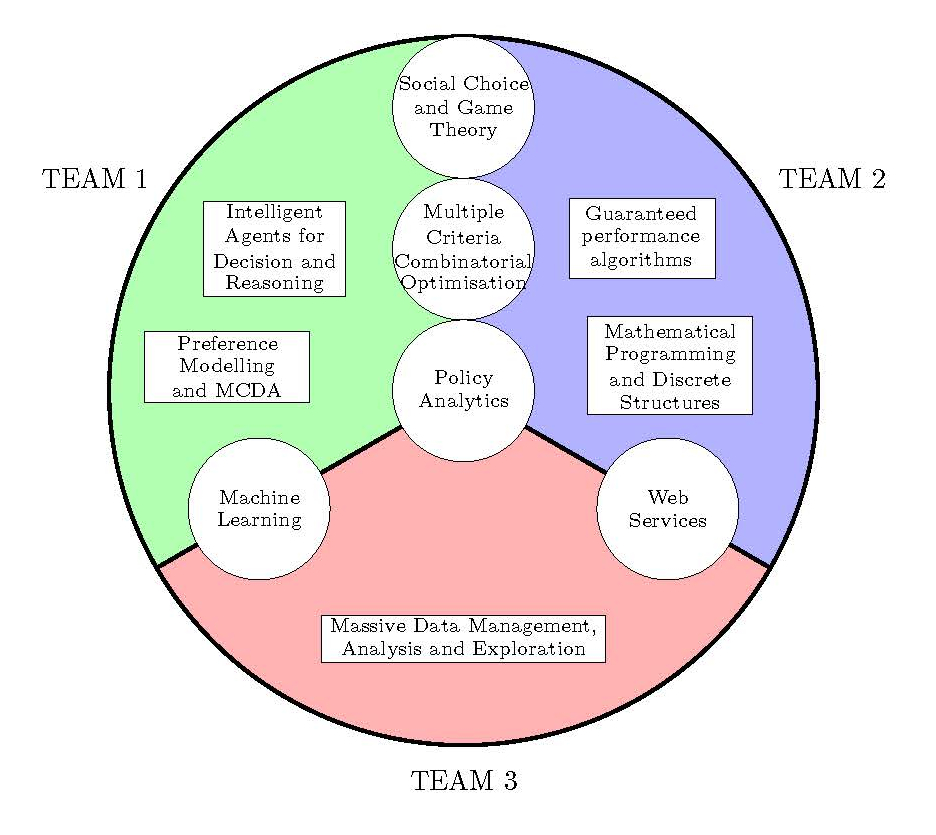
\includegraphics{organisation-en.jpg}}
%  \caption{Organisational chart of the LAMSADE structure}\label{organisation-en}
%\end{table}

\begin{figure}
	\centering
	\begin{tikzpicture}[scale=1.5]

%\draw [very thick,black,fill=gray!20](0,0) circle (3) ;

\draw [very thick,fill=red!30](3 * 0.866,3 * -0.5) arc (330:210:3) -- (0,0) -- cycle;
\draw [very thick,fill=green!30](3 * -0.866,3 * -0.5) arc (210:90:3) -- (0,0) -- cycle;
\draw [very thick,fill=blue!30](0,3) arc (90:-30:3) -- (0,0) -- cycle;
%\draw [very thick,fill=gray!45](0,3) arc (90:-30:3) ;


%\draw [thick] (0,0.60) -- (0,1.25) ;
%\draw [thick] (0,3) -- (0,2.75) ;



\draw [thick] (0.60 * -0.866,0.60 * -0.5) -- (1.4 * -0.866,1.4 * -0.5) ;
\draw [thick] (2.6 * -0.866,2.6 * -0.5) -- (3 * -0.866,3 * -0.5) ;


\draw [thick] (0.60 * 0.866,0.60 * -0.5) -- (1.4 * 0.866,1.4 * -0.5) ;
\draw [thick] (2.6 * 0.866,2.6 * -0.5) -- (3 * 0.866,3 * -0.5) ;


\draw [fill=gray!00] (0,0) circle (0.60) ;
\draw (0,0.1) node{{\scriptsize Policy}} ;
\draw (0,-0.1) node{{\scriptsize Analytics}} ;

\draw [fill=gray!00](0,2.4) circle (0.6) ;
\draw (0,2.6) node{{\scriptsize Social Choice}} ;
\draw (0,2.4) node{{\scriptsize and Game }};
\draw (0,2.2) node{{\scriptsize Theory}} ;


\draw [fill=gray!00](0,2.2-1) circle (0.6) ;
\draw (0,2.5-1) node{{\scriptsize Multiple}} ;
\draw (0,2.3-1) node{{\scriptsize Objective}} ;
\draw (0,2.1-1) node{{\scriptsize Combinatorial}};
\draw (0,1.9-1) node{{\scriptsize Optimisation}} ;



%\draw (1.1,1.1) rectangle (1.9,1.9);
%\draw (1.5,1.5) node{{\tiny Programmation }} ;
%\draw (1.5,1.3) node{{\tiny Math\'ematiques}} ;

\draw [fill=gray!00](1.05,-0.2) rectangle (2.45,0.63) ;
\draw (1.75,0.5) node{{\scriptsize Mathematical }} ;
\draw (1.75,0.3) node{{\scriptsize Programming}} ;
\draw (1.75,0.1) node{{\scriptsize and Discrete}} ;
\draw (1.75,-0.1) node{{\scriptsize Structures}} ;


\draw [fill=gray!00](0.9,0.95) rectangle (2.13,1.63) ;
\draw (1.5,1.5) node{{\scriptsize Guaranteed }} ;
\draw (1.5,1.3) node{{\scriptsize performance}} ;
\draw (1.5,1.1) node{{\scriptsize algorithms}} ;


\draw [fill=gray!00](-1.2,-2.3) rectangle (1.2,-1.9) ;
\draw (0,-2.0) node{{\scriptsize Massive Data Management,}} ;
\draw (0,-2.2) node{{\scriptsize Analysis and Exploration}} ;

%\draw (0.9,-2.0) node{{\tiny Services}} ;

\draw [fill=gray!00](-2.7,-0.1) rectangle (-1.3,0.50) ;
\draw (-2.0,0.4) node{{\scriptsize Preference }} ;
\draw (-2.0,0.2) node{{\scriptsize Modeling }} ;
\draw (-2.0,0.0) node{{\scriptsize and MCDA}} ;

%\draw (-1.8,1.0) node{{\tiny Optimisation}} ;
%\draw (-1.8,0.8) node{{\tiny Multicrit\`ere}} ;

\draw [fill=gray!00](-2.2,0.8) rectangle (-1.0,1.6) ;
\draw (-1.6,1.5) node{{\scriptsize Intelligent }} ;
\draw (-1.6,1.3) node{{\scriptsize Agents for }} ;
\draw (-1.6,1.1) node{{\scriptsize Decision and}} ;
\draw (-1.6,0.9) node{{\scriptsize Reasoning}} ;

\draw [fill=gray!00](-1.73,-1) circle (0.6) ;
\draw (-1.73,-1.1) node{{\scriptsize Learning}} ;
\draw (-1.73,-0.9) node{{\scriptsize Machine}} ;

\draw [fill=gray!00](1.73,-1) circle (0.60) ;
\draw (1.73,-0.9) node{{\scriptsize Web}} ;
\draw (1.73,-1.1) node{{\scriptsize Services}} ;

\draw (3.6 * -0.866,3.6 * 0.5) node{TEAM 1} ;
\draw (3.6 * 0.866,3.6 * 0.5) node{TEAM 2} ;
\draw (0,-3.3) node{TEAM 3} ;


\end{tikzpicture}

	\caption{Organisational chart of the LAMSADE structure}\label{organisation-en}
\end{figure}

The three teams of LAMSADE (Decision, Algorithms/Optimisation and Data Sciences) have essentially a mission of scientific animation (seminars, lectures, long term policy etc.) and receive a budget from the general budget of the unit (more details at section \ref{Management}). The research mission of the unit is accomplished by the 10 research projects:
\begin{itemize}
\item Preference Modeling and Multiple Criteria Decision Aiding;
\item Intelligent Agents for Decision and Reasoning;
\item Multiple Objective Combinatorial Optimisation (MOCO);
\item Machine Learning;
\item Massive Data Management, Analysis and Exploration (MADAX);
\item Web Services;
\item Mathematical Programming and Discrete Structures (Mathis);
\item Guaranteed Performance Algorithms (AGaPe);
\item Games and Social Choice: Axiomatic and Computational Aspects;
\item Policy Analytics.
\end{itemize}
These projects are aimed to conduct fundamental and applied research towards long term scientific or societal challenges.

Until recently the unit did not require any specialised computer equipment, the existing servers and network being sufficient. The establishment of the Data Sciences team and the more recent deep learning experiments conducted within the Intelligent Agents project pushed the unit to invest in the creation of a ``Big Data Cluster'' (co-funded by the LAMSADE, the CEREMADE and the MIDO Department, and managed by the LAMSADE) as well as to acquire dedicated hardware for deep learning experiments.

The unit is located at the main campus of Université Paris-Dauphine, and currently occupies 40 offices. However, this hardly covers our needs in individual and collective work space, the most critical situation concerning the PhD students and the post-docs. Equally importantly, these offices are still scattered in the building (two at the 2nd floor, eight at the 4th floor and thirty at the 6th floor), with some obvious negative consequences for the collective life of the unit. Unfortunately, until today the university has been unable to give a long-term satisfactory reply to our demand for a more appropriate location of our activities.

\subsection{Workforce and resources of the unit}\label{workforce}

This section is divided in three parts: the first one concerns the permanent scientific staff as well as the administrative one; the second one concerns the PhD students and the post-docs; the third one concerns the global resources of the LAMSADE.

\begin{table}
  \centering
   \scalebox{0.65}{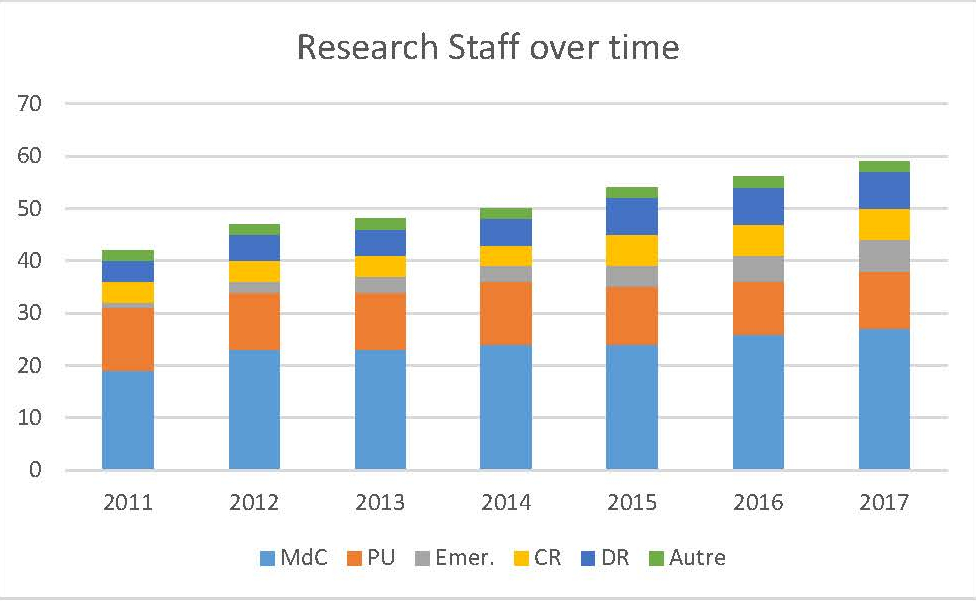
\includegraphics{staffovertime.jpg}}
  \caption{Evolution of research staff since the last report}\label{stafovertime}
\end{table}

Table \ref{stafovertime} presents the evolution of the permanent scientific staff of the unit. However, it does not explain the whole mobility process that has affected the LAMSADE for the last five years. In 2011 (when the last report was presented) the unit had 42 permanent scientific members, divided as follows: 19 associate professors (of which 3 belonging to other universities), 12 full professors (of which 1 belonging to another university), 4 CNRS junior researchers, 4 CNRS research directors, 1 emeritus, and 2 other researchers. At the time the present report is written, the LAMSADE has 56 permanent scientific members: 26 associate professors (among which 3 `externals'), 10 full professors (among which 1 `external'), 6 CNRS junior researchers, 7 CNRS research directors, 5 emeritus and 2 others, and with certainty will have 59 permanent scientific members in 2018 and 60 in 2019. During these 5 years, the LAMSADE presented on average more than 10 candidates annually for CNRS positions. As a result, we have seen the arrival of 3 CNRS research directors and 2 CNRS junior researchers (4 of these new CNRS personnel not being computer scientists). Meanwhile, 4 full professors retired (3 of which have been replaced or will shortly be, and one, in management science, has not been replaced by someone belonging to the LAMSADE), 5 associate professors left (4 of which were promoted to full professors\footnote{Université Pierre et Marie Curie, École de Mines de St. Etienne, École de Mines de Nancy, University of Freiburg in Switzerland}, and one moved to the private sector; all but one have been replaced), 5 more associate professors arrived (due to the retirement of 6 associate professors in computer science who were not members of the LAMSADE, since they did not have a research activity). All recruitements have been `externals' (no local PhD student was hired as associate professor, and no local associate professor was promoted to full professor), and for a large part international\footnote{2 full professors arrived from Université Paris Sud and one is on arrival from Université Paris 13. The 11 Associate professors recruited in this period arrived from post-doc positions: 3 from Japan (Universities of Tokyo and Kyoto), 2 from ILLC in Amsterdam, and 1 from Paris 13, from École Polytechnique, 1 from University of Manchester, 1 from INRIA Nantes, 1 from Université d'Orleans and 1 from University of Luxembourg}. Unfortunately, there has also been a recruitement by the university of a local PhD student, reason for which this colleague, although being a computer scientist, is not a member of the LAMSADE. At present, the unit hosts mosts of the computer scientists of Dauphine (more precisely, all of them but two), plus 6 CNRS scientists who are not computer scientists (essentially economists and management scientists). Summarising: in 5 years the LAMSADE renewed more than one third of its permanent scientific staff, giving at the same time a strong impulse to its scientific innovation and moving its median age towards the 30s (see the age line in table \ref{ageline}). It is important to note that at the beginning of the period under report the LAMSADE had 7 administrative staff working for the equivalent time of 5. Today the unit has 5 administrative staff, all of them occupied 100\% of their time (which thus has remained constant over time). Among these 5, 2 are permanent CNRS staff (one secretary and the computer engineer of the unit), 1 is a permanent employee of Dauphine (a secretary) and two are employees under contract (a secretary and the head of the administrative staff of the LAMSADE).

\begin{table}
  \centering
   \scalebox{0.65}{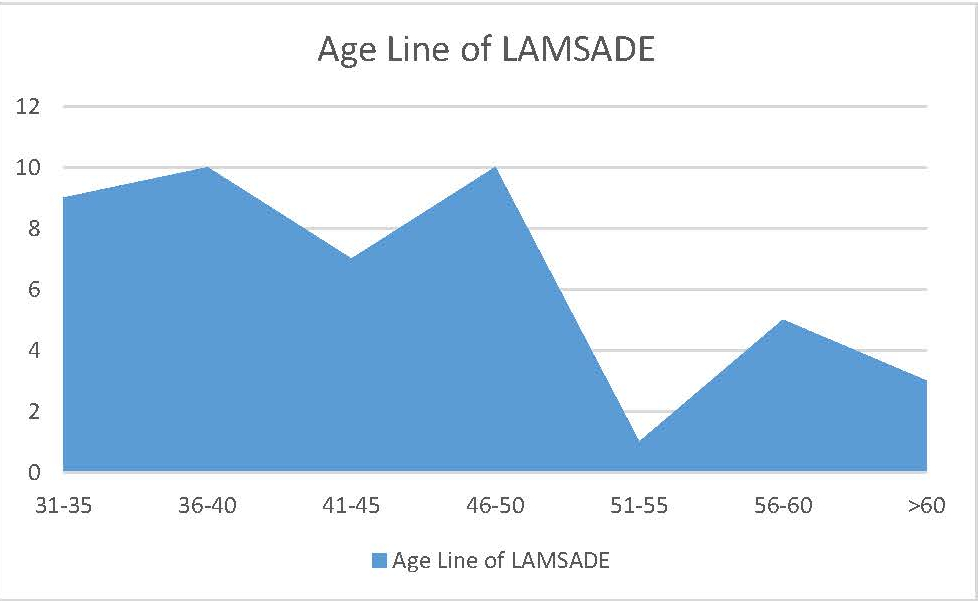
\includegraphics{ageline.jpg}}
  \caption{Age line of the research staff in LAMSADE}\label{ageline}
\end{table}

\begin{table}
  \centering
   \scalebox{0.65}{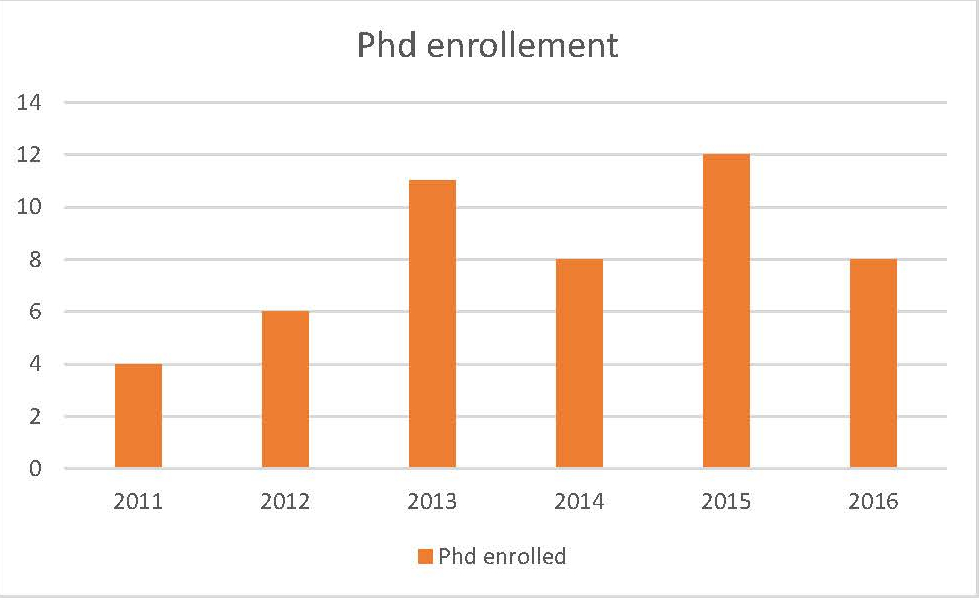
\includegraphics{phdenrollement.jpg}}
  \caption{PhD students enrolled since the last report}\label{phdenrol}
\end{table}

During the same period we undertook a serious effort to increase our capacity to tutor PhD students, by inciting the 
associate professors to defend their ``habilitation à diriger des recherches'' (HDR). Indeed, during these years, 8 among our Associate Professors and CNRS researchers obtained their HDR and at least two more are expected to do so before the end of 2017. This increased tutoring capacity joined to a global effort to attract more PhD students allowed to move our annual recruitement of PhD students to an average of 10 annually. Table \ref{phdenrol} shows the evolution of new PhDs every year (some differences over the years are due to the fact that some PhDs funded by industrial contracts actually start in the middle of the academic year, but are counted sometimes for the following year). Overall we had 46 new PhD students (of which two in management science and one in mathematics, the rest in computer science), with a strong concentration at the last years as a result of our policy.

\begin{table}
  \centering
   \scalebox{0.65}{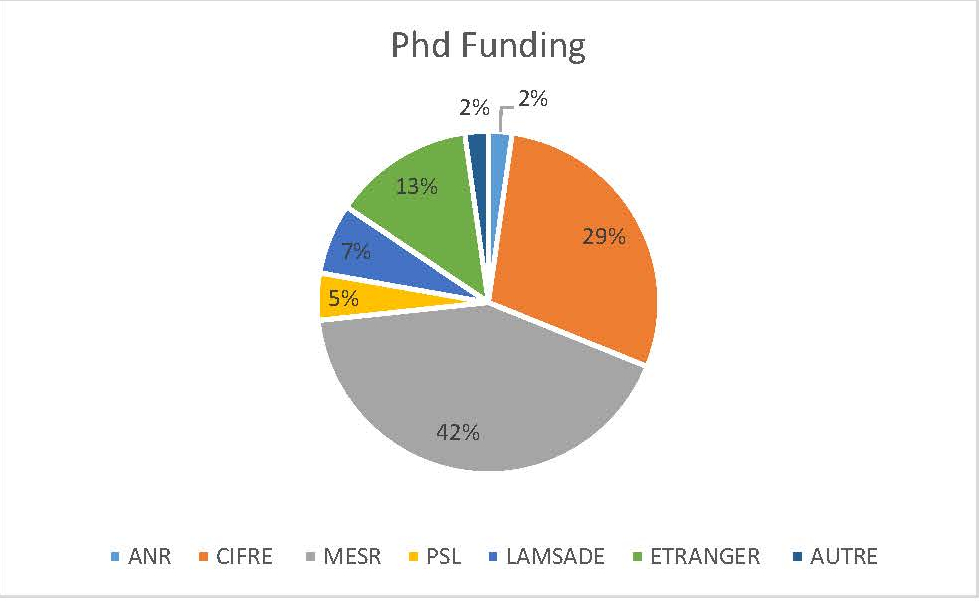
\includegraphics{phdfunding.jpg}}
  \caption{Distribution of PhD funding}\label{phdfund}
\end{table}

These 46 new PhD students have been funded in various ways (there are no non-funded PhD students in the unit). The distribution of the different funding sources can be seen in table \ref{phdfund}. As expected, the largest source remains the scholarships offered by the University through the Doctoral school and more recently by PSL. However, the second more important source are industrial contracts (CIFRE type), this type having become increasingly important during the last two-three years. The third source are PhDs funded by foreign governments, most of the time under co-tutoring agreements (Tunisia, Italy, Burkina Faso, Brazil). It is also worth noting that the LAMSADE has been able to fund 3 PhDs using its own funds (more details in section \ref{Management}). From 2013 on, we introduced a new competitive scheme for the recruitement of PhD students, which is now running in a very satisfactory way, attracting students at an international level (more details in section \ref{policy}).

\begin{table}
  \centering
   \scalebox{0.65}{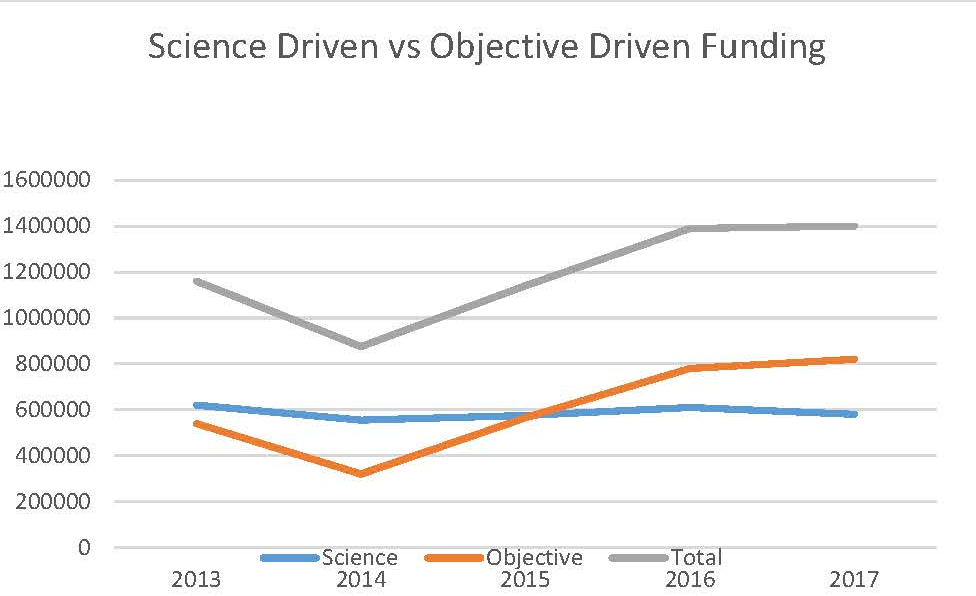
\includegraphics{globalfunding.jpg}}
  \caption{Global funding trends}\label{global}
\end{table}

The LAMSADE has an overall wealthy financial situation. However, in order to explain the global funding diagram presented in table \ref{global}, we need to explain how these figures have been obtained. The starting point has been the expenses of the unit: the everyday life, the research expenses (essentially missions, workshops and hardware) and most important the funding of the PhD students and the post-docs (it should be noted that in these 5 years the LAMSADE occupied 11 post-docs for periods going from 6 months to 2 years). Such expenses have been covered by different sources of income: the general funding coming from the University and the CNRS, the funding obtained competitively through projects (8 ANR projects, 7 PEPS of which 4 JCJC, 6 PSL projects) and the funding obtained directly, but most of the time indirectly, from industrial partners (more than 20 CIFRE contracts plus 5 direct research contracts). In counting the income generated we decided to include the indirect income corresponding to the funding of the PhD students, since this represents a non-negligible effort done by our members in order to secure such funds. The result is a global funding merging the direct funds and indirect ones. These are separated in two categories: the funds obtained on the basis of our scientific reputation and mission (science driven funding) and the ones obtained either through competitive funding or through industrial contracts (objective driven funding). Table \ref{global} shows the evolution of this funding over the last five years. The key figures to bear in mind from this table are: \\
 - the LAMSADE has an overall ``budget'' of approximately \EUR{1.4M}, regularly increasing every year; \\
 - the traditional competitive funding through the ANR has been in large part replaced by the funding from PSL; \\
 - there has been a sharp increase in the last three years of industrial funding essentially through CIFRE contracts (there have been more than 20, most of them recent ones).

As already mentioned, the financial situation of the unit is comfortable at the point to be able to fund on its own resources 3 PhD grants. This, however, should not conceal the fact that a large part of this ``wealthiness'' is obtained through contracts, (relatively) easy to negotiate, but with a limited horizon (for more discussion on this point see section \ref{swot}).

\subsection{Scientific policy}\label{policy}

The missions the LAMSADE, as stated when it was evaluated five years ago, can be summarised as follows:
\begin{itemize}
\item strengthen the international position of the unit as one of the European leaders in Decision Sciences and Technologies;
\item improve the internal life in the laboratory, by increasing participation and commitment;
\item help the early stage researchers to make their way in their careers;
\item make the LAMSADE a nice place to work, to study and to produce good science.
\end{itemize}

In order to strengthen our international recognition, we have been pursuing two main directions. The first one has consisted in strengthening our role of research communities creators and animators. Our positioning in algorithmic decision theory, game theory, computational social choice, parametrised complexity, polyhedral combinatorial optimisation, graph theory among the European leaders is a fact. The second direction has consisted in pursuing both excellence and internationalisation to all of our recrutement actions (PhD students, post-docs or new colleagues). Under such a perspective, we are very proud that we manage to attract people from all over the world to come study with us, to work with us or even to visit us. The LAMSADE is an international crossroad.

However, this policy would have given only partial results if not completed by our clear investment in Data Sciences. The creation of the third team of LAMSADE around this topic, and the recruitement of several new colleagues (6 out of 9) has been a collective effort the whole unit decided to undertake despite the risks and the difficulties such a decision implied. Our investment already starts paying positioning the unit at an international level also in this area.

It has been a deliberated policy to improve and better organise the internal life of the unit: approaching a global size of 100 and with three large teams, and taking into account that more than one third of our scientific staff has been renewed during these years, a clear regulation of our internal life was necessary. This mainly concerned the use of our common resources: funding, PhD scholarships and positions available for temporal recruitements (invited professors or assistant professors) and for permanent ones. The regular meetings of the Council allowed to discuss and establish clear rules for this purpose. It has been a long process, which is not yet achieved since we need to update and revise our rules as we cumulate feedback. It has not been always simple to conduct this process (through misunderstandings, misinterpretations and errors ...), but the rules of our internal life now exist and work.

The LAMSADE continued in these years to pursue its policy aiming at helping the early stage researchers to integrate the scientific life of the unit. For this purpose we have a special fund dedicated to the PhD students and to the colleagues who have just joined us. This allows to cover scientific missions otherwise impossible to undertake. Further on we decided, when the PhD grants are distributed, to give the priority to proposals coming from our ``young'' associate professors in order to give the opportunity to start directing a PhD student (this being one of our fundamental missions).

The structure of the unit has already been presented in Section \ref{presentation} and in Table \ref{organisation-en}. The three teams of the unit are aimed to conduct essentially research animation (seminars, invitations etc.) and to federate colleagues sharing a broad scientific area within the LAMSADE area. The ten projects instead are aimed to conduct long-term research activities on a given subject, which we expect to last for a sufficiently long period (such as 10 years). The projects are aimed to raise their own resources. These projects do not necessarily ``belong'' to a team. Actually five of them intersect two or even three of the teams both in terms of research subjects, but also in terms of people involved (it is the case that people from several teams contribute to the scientific life of the projects).

In choosing our research priorities, we consider the following guidelines: \\
 - allow the LAMSADE members to pursue their own individual research interests; \\
 - provide a scientific identity to the unit justifiable and compatible with the identity and policy of Dauphine (and more recently PSL); \\
 - fulfill the high standards in terms of quality and management required by the CNRS; \\
 - maintain at least 10 years of scientific advantage (in terms of knowledge) with respect to the demand of the society; \\
 - be able to respond positively to the challenges our society (France, Europe, World) present us.

As a CNRS research unit, our fundamental mission is to conduct fundamental research. However, we need to consider two constraints in pursuing this mission. The first derives from the fact that funding for fundamental research is decreasing. Or to be more precise: funding for science-driven research is decreasing. We define science-driven research as activities guided by our knowledge, training, experience and intuition as researchers: research which is not expected to deliver a precise result, but to advance knowledge and attack challenges which most of the people and the organisations around us ignore or do not consider actual. However, it is this type of research that delivers the results and the knowledge in order to handle the problems our societies will face 10 or more years from now. Given the present situation, where this type of research is generally undervalued, we decided to dedicate part of resources in funding ``science-driven'' PhD grants (besides the ones offered by the University). We have been able to fund 3 such grants. The second constraint is related to the specific nature of our research in decision sciences and technologies. Our objective is to improve how people (and automatic devices) decide as well as how analysts help people (and automatic devices) to decide. Decision making and aiding decision making are essentially empirical activities and the inputs for innovation in our field have always been offered by real life. Under such a perspective it is essential for a unit like the LAMSADE to keep a constant contact with the demand for decision support the society around us presents. For this purpose we consider the societal challenges around us as research challenges and we dedicate part of our research being implied in real cases of decision aiding (this being any among models, algorithms, data structures, services etc.). The result of these two constraints is that the LAMSADE has a policy of wise equilibrium between science-driven and objective-driven (reply to a precise challenge) research.

In order to conclude our policy presentation, we may mention that it has always been a priority trying to make the LAMSADE a nice place to work and study. Besides enabling our members to conduct their research with as less hassle as possible we try to promote cooperation, mutual respect and understanding, equal opportunities and a lively environment for discussion and exchange of ideas. The fact that we receive every year a very high number of foreign visitors contributes very much in this direction. However, we may also mention that we also try to promote an idea of research as ``having fun'', since this is an essential component for the creativity research requires. We do serious research, but we are very proud not to be always serious!

\section{Production}\label{secproduction}

A global overview of the scientific production of the LAMSADE can be seen on Table \ref{production}. In this table we counted only peer reviewed journals, selective international conferences, books, chapters in books and edited proceedings and volumes. Quantitatively, the unit has a practically constant production of a good level: considering an average presence of 50 permanent scientists within the LAMSADE during the period considered we get an average production of 3 publications per scientist per year.
\begin{table}
  \centering
   \scalebox{0.65}{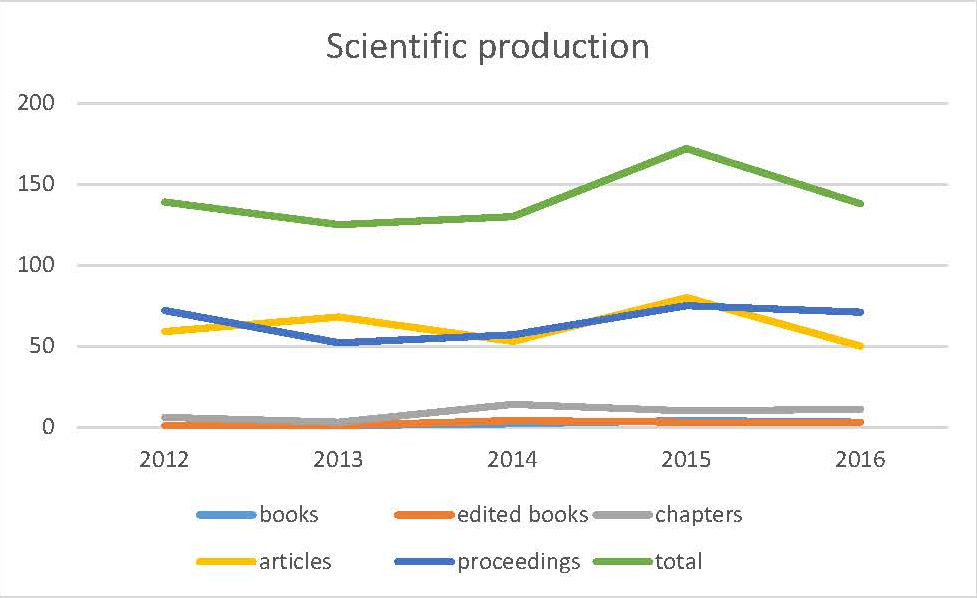
\includegraphics{production.jpg}}
  \caption{Global scientific production of the LAMSADE}\label{production}
\end{table}

To this result we may add the fact that the LAMSADE members are present in the editorial board of more than 30 international journals (one editor in chief) mainly in the area of Operational Research and Decision Analysis and in an uncountable number of scientific committees of international conferences including some among the more prestigious ones. The members of the LAMSADE have been invited to give talks/lectures/tutorials to more than 100 conferences and workshops around the world (not counting the personal invitations for seminars and visits). Let us also mention that during these years the LAMSADE received the visit of more than 80 foreign colleagues from more than 35 different countries for approximately 100 months of invited professor. Last, but not least during this period there have been 36 PhD defenses (the average duration of a PhD thesis being 3,9 years) and 8 HDR ones (for a discussion about the job destination of the former PhD students the reader can see Section \ref{swot} and Table \ref{phdjobs}).

However, these results do not reveal the qualitative evolution of our scientific production. While we kept a constant quantitative production the quality of our papers sharply increased. Journals such as Mathematical Programming, INFORMS Journal of Computing, Artificial Intelligence or JAIR now regularly publish our results, while top tear conferences such as IJCAI, AAAI, AAMAS, ICALP, ESA, EDBT, WWW are now regularly visited by our researchers presenting their results.

A detailed presentation of the scientific achievements of the three teams can be seen in \cref{team1,team2,team3}. In the following, however, we give a rapid outlook of the major scientific achievements of the LAMSADE in the last 5 years.

\vspace{5mm}

1. The axiomatic characterisation of bibliometric indices as well as the axiomatisation of preference aggregation procedures based on the concordance/non discordance principle (\cite{Bouyssou2015A-634565}). \\
2. The GRAVE algorithm, designed as a generalisation of the well known RAVE algorithm which greatly improves its performance in many games; see \cite{Cazenave2015Generalized-1222829}). \\
3. The Handbook on Computational Social Choice (presented in 2016): in this book which is now a landmark of this research topic, one of the editors is a LAMSADE members, 3 out of the 19 chapters of the book are co-authored by members of the LAMSADE, while 8 others by invited professors of our unit (sometimes during their stay at LAMSADE; see \cite{HBCOMSOC2016}). \\
4. Two nice real world applications of our research: the first concerning the use of MCDA methods in order to evaluate different layouts of the new rail line from Paris to Normandie and the second concerning the use of inverse Banzhaf indexes in order to find the proportion of seats for each Institution within the Academic Council of PSL (the actual distribution of seats is the one our method suggested). \\
5. In the area of Complexity and Approximation two results can be considered as outstanding: \cite{DBLP:journals/algorithmica/BonnetE0P15} proposes a formal framework for super-polynomial approximation (mainly sub-exponential and parameterized) and provides inapproximability results for paradigmatic problems (as maximum clique, dominating set, etc.) in this framework, while \cite{Karpinski2015New-1298222} tightens the known inapproximability bounds for the Metric Travelling Salesman Problem. \\
6. Two breakthrough contributions which we recently contributed in Mathematical Programming. In \cite{DBLP:journals/mp/AissiMMQ15} the multiobjective and parametric versions of the global minimum cut problem in undirected graphs and bounded-rank hypergraphs with multiple edge cost functions are studied. They proved that for a fixed number of edge cost functions, the total number of supported non-dominated cuts is bounded by a polynomial in the numbers of nodes and edges. In \cite{Cornaz2014Chromatic-623556} the quality of Lov\'asz theta function, as a bound for colouring, is improved using graph theoretical tools. \\
7. A main contribution in the field ``Multiobjective combinatorial optimization'' is the introduction of the concept of search region~\cite{Klamroth2015On-634730,Dachert2017Efficient-1250848} which enables the design of efficient algorithms generating exactly or approximately the non-dominated set.  Another original stream of research deals with the generation of the preferred solutions in the sense of aggregation models such as OWA~\cite{Galand2012Exact-610325}, Choquet~\cite{DBLP:conf/ijcai/GalandLP13}, Lorenz~\cite{Galand2015Exact-1052488} or a partially defined weighted sum~\cite{Kaddani2017Weighted-1232001}. \\
8. A major advance in data integration has been done by showing that the cost of ensuring good quality of integration can be reduced dramatically using a small number of feedback instances solicited from end users \cite{Belhajjame2013Incrementally-904545,DBLP:journals/dpd/BelhajjamePHF15}. In the context of BigData, the PAQuery systems has been proposed \cite{DBLP:conf/sigmod/Camacho-RodriguezCM14, DBLP:journals/tkde/Camacho-Rodriguez15}, providing the first formal specification and implementation of a powerful compilation technique from the XQuery query language to PACT, a powerful extension of MapReduce. \\
9. Within the context of a collaboration with Google (Google Brain at NYC and Google Research at Palo Alto), Nvidia, Columbia University, Courant Institute, and CEA List, we proposed in~\cite{Bojarski2017Structured-1259771} a new framework for speeding up several machine learning algorithms (e.g. kernel approximations, deep learning, LSH, etc.) with almost no loss of accuracy. In the context of Computer Games, we continued our seminal works on Monte Carlo Tree Search (MCTS) and proposed significant improvements to the architecture of the deep neural networks of AlphaGo~\cite{cazenave2017residual}. In the context of generalization of regret minimization to the Blackwell approachability setup,~\cite{FLP2016} shows that unlike in standard online learning literature, the necessary or sufficient conditions for the anytime version of this problem are drastically different than those for the fixed horizon. \\
10. Based on our experience on process mining and matching, we participated in writing a monograph (published by Springer) \cite{DBLP:books/sp/BeheshtiBSGMBGR16} that surveyed approaches and tools for process analytics (co-authored with experts in the field from UNSW Australia, IBM Almaden Research Center,... ). Concerning services, we have proposed several solutions and a complete analysis of complexity and models for service discovery, composition and execution problems, taking into account non-functional properties  \cite{GMMM17, AngaritaArocha2016Modeling-1159056}. In a seminal work~\cite{Abu-Khzam2015On-1017005}, we have a comprehensive study and prove of the exact complexity of the service selection problem by taking into account QoS criteria for single and multi-criteria instances.\\
11. An important breakthrough has been the establishment of a new interdisciplinary research subject: policy analytics (\cite{Belton2013Policy-624015}) aiming at improving decision aiding in designing implementing and evaluating public policies. A new national (\url{www.gdr3720.fr}) and international scientific community are now under construction.
\vspace{5mm}

Overall the LAMSADE is proud of the work accomplished during these years. However, there are a number of highlights for which we are particularly proud and we may illustrate in the following as examples of our achievements.

1. In 2014 the LAMSADE celebrated 40 years of activities (it has been created in 1974). We organised during the year 4 lectures involving Google, Frédérique Ségond, Christos Papadimitriou and Hervé Moulin, all of which had a great success. These lectures contributed significantly to the scientific reputation of the unit (both within our strict environment and beyond it). This visibility has been completed by the delivery of three Doctor Honoris Causa to three outstanding colleagues: Fred Roberts, Christos Papadimitriou and Claudia Bauzer Medeiros. \\
2. In 2015 we received 4 CNRS researchers who are not Computer Scientists. It has been a massive sign of trust from the CNRS and at the same time a huge challenge for the LAMSADE: become able to integrate different disciplines under the Decision Sciences and Technologies perspective. We are proud to see this challenge turning into a success (completing other interdisciplinary initiatives such as the Master in Peace Studies). \\
3. In 2016 the LAMSADE undertook a large restructuring ending with the establishment of the Data Sciences team and the appearance of new projets enabling the appropriate visibility of cross-laboratory research subjects such as social choice, game theory or machine learning. It has been the end of a process started in 2012 when the recrutement policy of the unit has been first discussed and is now continuing as a challenge for the whole LAMSADE for the future. \\
4. In 2016 Bernard Roy received the EURO Distinguished Service Medal strengthening the already well known reputation of the LAMSADE in the domain of Operational Research and Decision Analysis (it should be noted that the LAMSADE is the only OR laboratory in Europe who has an EURO Gold Medal, 2 former presidents of EURO and now the EDS Medal). The same year Stéphane Airiau coauthored the paper which won the ``Best Paper Award'' at the prestigious AAMAS conference (\cite{Airiau2016Rationalisation-1088325}). \\
5. In 2017 we received a very prestigious recognition of our efforts. Jérôme Lang and Eunjung Kim received the CNRS silver medal and bronze medal (respectively) in Computer Science. It is the first time that the same research unit receives the same year two such distinctions. It should be noted that during the period under consideration Cristina Bazgan and Vangelis Paschos were recipients of two IUF grants (junior and senior respectively). \\
6. During this period we increased our efforts in order to enhance and improve our outreach both for specialised audiences (other than computer science) and the general public. Despite our natural aversion for too much advertising we have been able to comunicate on several ``hot subjects'' including Artificial Intelligence and Machine Learning (thanks to our colleague Tristan Cazenave who now regularly appears on the media for his expertise in AI). However, the single project for which we are very proud is the video we produced in order to celebrate our 40 years. We have been asked to prepare an institutional advertisement of our activities and we ended preparing an unconventional story about who we are and what we do. We are still able to have fun and to make a joke of ourselves in this laboratory.
%2. Scientific production and activities (for the unit, and next for each team and/or theme of the unit)
%Sections 2-5 will be filled first for the whole unit, and then for each team and/or theme of the unit.
%Scientific output
%The unit (or the team /theme) will give a global overview of the scientific outputs of the current contract.
%Quantitative data
%Quantitative data on the whole production and activities of the unit or team/theme are to be given in the Excel file “Données du contrat en cours”, Table 5, “Scientific production and activities”.
%Selected production and research activities
%Please provide a selection of the unit or team/theme scientific production and activities (in appendice 4, see page 4). Concerning the scientific production (paragraphs I, II and II), the list has to be limited to the most significant 20%.
%The complete list of production and activities of the unit or team/theme needs to be provided (for example on a website) to the committee upon request.
%Highlights
%Here, the unit or team/theme will briefly discuss a restricted number of highlights concerning any of items of the scientific production and research activities.
%Please adjust the number of highlights to the size of the unit or team/theme.

\section{Management}\label{Management}

The management structure of the LAMSADE is summarized on Table \ref{organigramme}. As usual happens there is a director (and a vice-director) a Council of the unit, an administrative team and three teams leaded by their respective coordinators.

\begin{table}
  \centering
   \rotatebox{-90}{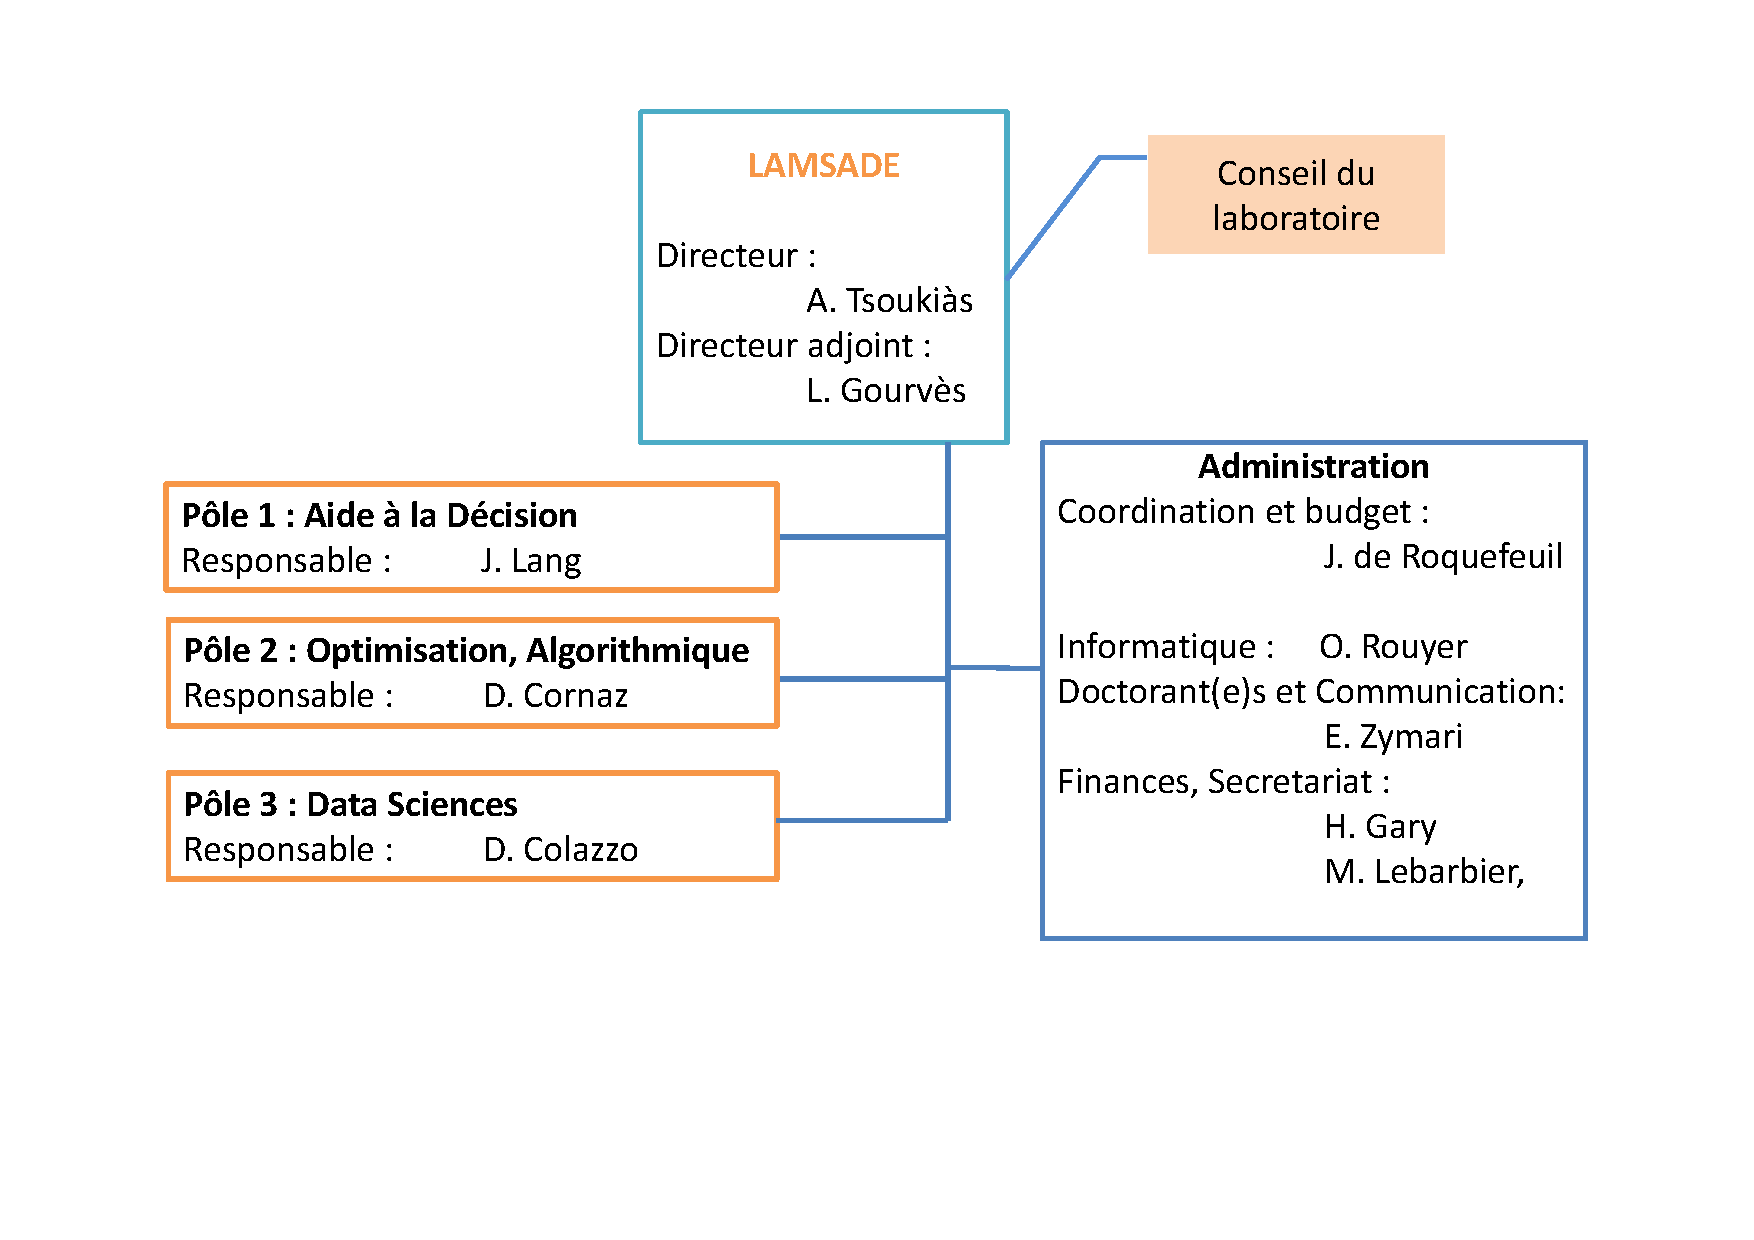
\includegraphics[height=\textwidth]{organigramme.pdf}}
  \caption{LAMSADE management structure}\label{organigramme}
\end{table}

The management of a research unit of the size of LAMSADE is relatively simple. First of all there are two major regular collective moments in the life of the unit: \\
 - the LAMSADE day, occurring usually at the beginning of spring, dedicated to scientific discussion, the presentation of the new colleagues, of new research projects etc.; a speed presentation (180 sec.) of the second year PhD students also takes place; \\
 - the general assembly (GA) of LAMSADE, occurring the third Tuesday of June, where the policy of the unit is discussed for at least one critical issue (training, scientific strategy etc.).

The organisation of the LAMSADE days started in 2012 and evolved during these years to the present format (stable since 2016) which seems to satisfy most of the members. It should be noted that in 2014 we did not organise the LAMSADE days due to the celebrations for the 40 years of the unit. The two main subjects discussed in the GA of the unit have been the creation of the Data Sciences team and the innovation of our training offer in Computer Science (on that last topic there have also been a couple of exceptional GAs).

The life of the unit is essentially organised by the 3 teams and the 10 projects. However, as far as management is concerned, the 3 teams regularly meet in order to discuss at a decentralised level topics related with the policy of the unit, while this is not the case of the projects. The teams mission is to animate discussions (seminars and policy issues). The teams also have a budget (\EUR{15K} annually coming from the general budget of the unit) which is expected to support missions and other scientific animation activities. On the other side the projects (5 of which are transversal to the teams; see Table \ref{organisation-en}) are expected to conduct research (most of the times through PhDs and Post-Docs), to organise scientific events and to contribute to the global fund raising of the unit. Under such a perspective the projects do not receive a regular budget from the general one (although may occasionally ask for some support), but they compete for a critical resource which are the PhD scholarships.

The unit is managed by the director (and the vice-director) assisted by the administrative staff in interaction with the Council of the unit. The latter is the typical consultative structure of all CNRS units: it is expected to be consulted on all critical issues of the unit's life. It is composed by 15 members (plus the co-director of MIDO and the administration responsible who are permanently invited): \\
 - the director and vice-director; \\
 - 9 elected members (7 among the scientific staff, 1 among the administrative staff and 1 among the PhD students); \\
 - 4 appointed by the director. \\
It meets 8 times during the year (always on Tuesdays at noon) on rolling dates which are now becoming stable. Besides discussing regular topics (budget, recrutements etc.) it also has a special mission: identifying every year the subjects for which we look for PhD candidates, organise the hearings of the candidates and prepare a ranking which is submitted to the Doctoral School. \\
For most of the everyday issues the direction and the staff are sufficient. Occasionally there are cases where an enlarged version of the direction meets including the three team leaders.

Parallel to the Council there is the CCR (a Representative Consulting Committee) required by the statutes of Dauphine and concerned by the hiring of scientific staff (in the case of LAMSADE in Computer Science). This Committee is led by the director of the LAMSADE, it is composed by 20 members (10 full professors or research directors and 10 associate professors or researchers), 16 of which are elected, 3 being appointed by the director, the director being also a member. This committee meets 3 times during the year: \\
 - in late autumn in order to fix the essential lines of any recrutement profile and to identify the person in charge of the selection committee (any long term policy issues are also discussed in this meeting); \\
 - in late winter in order to approve the profile of any recrutement and the selection committee; \\
 - in early summer in order to rank the applications for invited professors and the applications for assistant (not permanent) professors.

As already mentioned the LAMSADE is one among the few research units in Computer Science with more than one third of its permanent scientific staff being women. We are very proud of this and we actively pursue ways aiming to maintain this situation with particular emphasis to all recruiting opportunities.

\section{SWOT}\label{swot}

There are multiple strengths at the LAMSADE. The unit has a well established identity (Decision Sciences and Technologies) which spans from our traditional subjects (Operations Research, Decision Theory, Algorithms, Artificial Intelligence) to the more recently added ones (Machine Learning, Database Management etc.), thus covering the whole range of Computer Science and Decision Sciences. We have a regular administration, clear rules for the distribution of all critical resources and a wealthy financial situation. We produce very good science and our international reputation has never been stronger. We have taken up an interdisciplinary challenge, which for the time being works fine with respect to all the disciplines with which we cooperate; more importantly, we attract researchers from other disciplines to come and work with us. We have also taken up the challenge to become more international, and this has also been a success. We attract colleagues from all over the world as well as PhD candidates. There is, however, one single strength for which we are proud and for which we consider the LAMSADE as unique: the fact to have created and contributed to create several international research communities. We do not only anticipate the scientific challenges (as any fundamental research unit should do), but we create the communities who will take care of them. Decision Sciences and Technologies is a niche domain requiring strong networking activities: the LAMSADE is at the unit of these networks.

There are also clear weaknesses. Undoubtedly the establishment of the new team has been unevenly perceived within the laboratory as there are obvious differences among the three teams. It is certainly unfair to compare a team established since the creation of the LAMSADE and one created only since 18 months. Besides and on the long run such differences are not expected to stand (the Data Sciences colleagues are doing an excellent work which will not take a long time to show the results), but for the time being these exist and could create frictions within the unit. To some extent, this is related to the low visibility our research projects presently have, an issue which needs to become a priority in the near future. However, there are two major weaknesses which need to be considered in the very near future. The first concerns the capacity of the unit to secure long term funding for fundamental research. The present financial wealthiness should not conceal the fact that this is secured thanks to short term objective driven contracts, easy to obtain, but far from representing the ambition that a unit like the LAMSADE should have. The second concerns the attractiveness of Computer Science training at Université Paris-Dauphine. Although this is an issue which concerns more the Department of Mathematics and Computer Science (MIDO) it is clear that the LAMSADE, representing de facto the whole Computer Science community of the University is directly concerned. The fact is that the attractiveness of Computer Science is unevenly distributed among the various training programs and we are yet missing a situation where our scientific reputation could be transformed to attraction for prospective students.

Which are the opportunities offered by the environment where the LAMSADE evolves? Under a contingent point of view this is a time where the knowledge owned by the unit is highly demanded by the society. The investments we did several years ago specialising the unit in areas at that time ``of little interest'' turned to be today a big advantage. At the time where the government considers for instance that the domain of Artificial Intelligence should become a national priority, we are proud to know that we are among the leaders in this area. The same applies to other domains such as Data Sciences, Analytics or the social responsibility of algorithms. There is a huge demand out there in the real world and we can catch it. On a longer run the fact that we showed our ability to conduct interdisciplinary research and to create new areas of scientific investigation at the edge of several disciplines corresponds to a demand of increasing scientific contamination and for new frontiers. We know we can handle such challenges. Last, but not least, the increasing internationalisation of training among European countries and the increasing mobility of students across Europe represents a huge opportunity for innovating our training programs and diversify our training offer policy with big potential positive impacts.

\begin{table}
  \centering
   \scalebox{0.65}{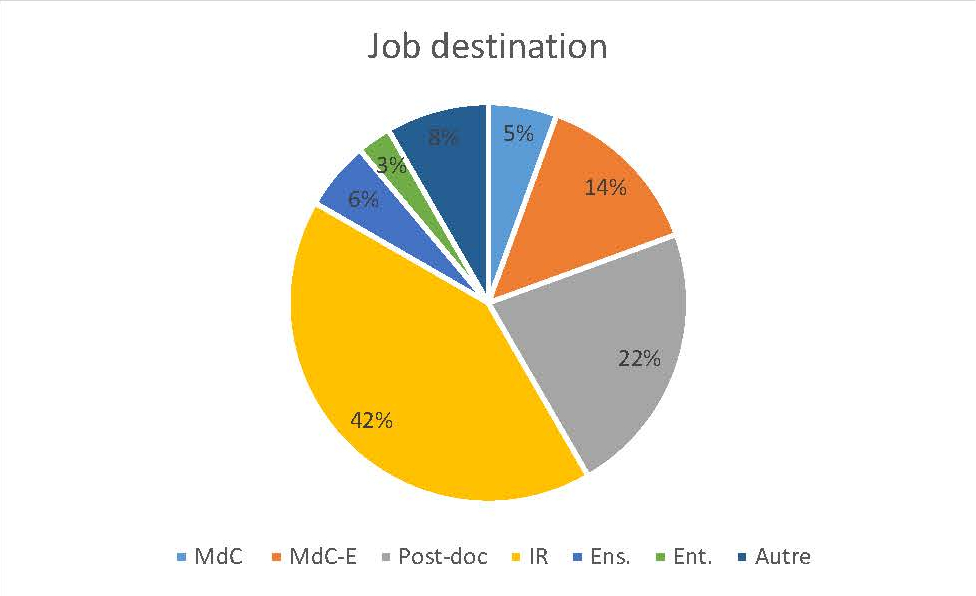
\includegraphics{phdjobs.jpg}}
  \caption{Job destination of PhDs}\label{phdjobs}
\end{table}

Certainly, there is a number of threats we need to consider. Some of them are completely out of our control: both at a national and at a European level there is a persistent policy of downsizing the research infrastructure (particularly the manpower both in research/training and in administration/support) and the science driven funding. At a certain point this will have dramatic effects. Our young colleagues have increasingly less opportunities to pursue their career (unless they turn to the private sector where there are certainly excellent offers from giants of the Computer Science and Decision Sciences business; it has been the case for one of our associate professors and for brilliant young PhDs who finally decided for this option). It is a trend confirmed by Table \ref{phdjobs}: the vast majority of our PhD students is in the private sector. Our research also is suffering: when the prior probabilities of being funded through a competitive call start falling beyond 20\% (sometimes less than 10\% or even less than 5\% ...) the expected utility of introducing an application is negative. If, as presently happens, obtaining an industrial contract is relatively easy, our researchers increasingly turn their eyes to these relatively ``short term'' objective driven research. But on the long run this is not sustainable: the replacement of ideas used with new ones is too slow and soon or later we will find ourselves with no new ideas ... A relatively more contingent and local threat is represented by the relatively modest size of Computer Science (as a discipline) within PSL. PSL de facto represents an important actor (for institutional reasons, for the volume of resources they manage, for the international impact it has), but Computer Science is a marginal subject and discipline within it. Although the two principal research units in Computer Science within PSL (the LAMSADE and the DIENS) have a large international reputation and recognition, their quantitative size is too small with respect to other disciplines and research fields. This requires an accurate strategy of scientific and interdisciplinary alliances, but this is a topic for our strategy section.

\section{Strategy}\label{strategy}

To a large extent, the strategy of the LAMSADE for the next five years derives from our SWOT analysis and the elements we highlighted while presenting the activity report of the unit. We may summarise our priorities in 5 specific areas where we need to concentrate our efforts during the next years: International Visibility, Computer Science Training, Dauphine and PSL, our structure and our funding, our human resources.

\begin{enumerate}
  \item \textbf{International Visibility}. The LAMSADE already has a strong international reputation. As already mentioned we do not only produce good science which is internationally recognised, but we also took several times the initiative to co-create and co-conduct national and international scientific communities. That said, it needs to be understood that, in several fields of the area of Decision Sciences and Technologies, international leadership is now expressed by large global private companies whose R\&D departments largely dominate in terms of size and resources most if not all university research units and departments. Under such a perspective a direct competition on mainstream subjects risks to be counter-productive and not sustainable on a long term. If the LAMSADE wants to be considered as one of the leading European units in this area (Decision Sciences and Technologies) it needs to focus on subjects which either escape the short to medium perspective of this type of competitors or correspond to societal needs and challenges underestimated and thus more or less ignored. In other terms, on the one hand we need to focus ever more now on our fundamental research subjects anticipating the scientific challenges at an horizon of 10-15 years (new optimisation methods, new schemes of algorithmic complexity, new models for learning etc.) and on the other hand we need to produce convincing results as far as critical societal problems are concerned (citizen participation, policy design, society polarisation, homeland security, just to mention a few of these).

      On these subjects and with such objectives we need to attract to the LAMSADE people from all over the world (PhD students, post-docs and scientific staff) willing to participate to our scientific adventure. At the same time we need to strengthen our presence and leadership to all communities where we are involved and foresee the creation of new ones (such as the one concerning the social responsibility of algorithms). We also need to take advantage of our interdisciplinary perspective in order to maintain an innovative perspective to the challenges in front of us.
  \item \textbf{Attractiveness of computer science training}. Despite the LAMSADE not being directly involved with the design of the training activities (these being delegated to the Mathematics and Computer Science Department: MIDO) it is obvious that any initiative concerning the training in computer science has a direct impact to the life of the LAMSADE. Having attractive computer science training programs means having good students to work with, a stimulating environment for consolidating knowledge, improving international visibility and attractiveness (after all we try to attract colleagues who are going to teach most of the times), expanding the outreach of our work.

      The subject has been discussed several times in the recent years in dedicated meetings of the computer scientists of Dauphine (which more or less corresponds to the members of the LAMSADE). There is an uneven attractiveness of the different training programs, there is an uneven visibility of these, but what is perhaps most important is that we do not present a global vision of what means for a young student to be trained in Computer Science at Dauphine. The result is that we still miss a global vertical program in Computer Science.

      Our aim is, in cooperation with our colleagues in CEREMADE and more generally MIDO, to design a more comprehensive and readable program in computer science (lasting 5 years, under different formats) including an horizontal training program in mathematics and computer science at the bachelor level. This is not the place where these ideas ought to be developed; we want to affirm our commitment for an innovative and attractive program in computer science (and in mathematics) at Dauphine.

      Besides this commitment, we need to quantify and improve the way through which computer science is taught in training programs which are not in computer science (management, economics etc.). Last, but not least, it is important to maintain our commitment to the interdisciplinary program of Peace Studies which has been created under our initiative and today presents a big success for the whole University and the PSL.
  \item \textbf{Dauphine and PSL}. When the previous evaluation exercice of the LAMSADE took place PSL was more a project than a reality. Today PSL is a strong reality and despite the problems all new endeavours have, we are expecting it to become a hard constraint to our everyday life as a research laboratory. We already mentioned that PSL can be seen both as an opportunity and as a threat. An opportunity because of the resources it mobilises, the international visibility that can add and the challenges it represents. A threat because of the relatively modest quantitative presence of computer sciences (and even less Decision Sciences and Technologies) within it. The practical risk is to see once again the computer science considered as a service and not as a discipline by itself. To some extent, this is an experience we had the early years within Dauphine, where Computer Science was relatively modest. There are three actions the LAMSADE can and has to undertake in order to strengthen its position and at the same time strengthen Dauphine and PSL as Global Higher Education and Research Institutions. \\
      1. The first consists in strengthening the relations and cooperation with the computer scientists within PSL (mainly the DIENS which is the other strong reality in computer science within PSL). We already have a number of joint projects, but regrettably there has been no coordination among the two units and this needs to be improved: we expect the discussions about the computer science training within PSL and the existing positive experiences may help in that direction. \\
      2. The second consists in further developing our interdisciplinary potential. Several among our research projects (Social Choice and Games, Policy Analytics) and training initiatives (Peace Studies) have a strong interdisciplinary nature which addresses forces beyond the computer scientists creating alliances (in Economics at ENS, in Management in École des Mines, in Social Sciences at EHESS) through which increase the awareness of the importance to have a strong component in Decision Sciences and Technologies within the PSL. \\
      3. The third consists in using our enormous international network in order to promote initiatives that could help on the one side the international recognition of PSL and on the other side to promote our research. Under such a perspective our recent initiative to establish a UMI implying PSL, CNRS and ANU is a typical action in this direction.
  \item \textbf{Structure and Funding}. The LAMSADE has now a stable structure which we do not expect to put under discussion in the following years. That said, it is natural to expect that the 10 scientific projets, through which we essentially produce our research, may look for more visibility, gain an increased autonomy and turn to be the essential units of the unit.

      On the one hand, this structure allows the members of the LAMSADE to participate to more than one project enabling them to pursue their scientific interests in a much more flexible way. On the other hand, this is a much more agile structure allowing to mobilise and attract ressources mainly through competitive funding. It also allows to adapt much better to the demands originating from societal challenges we may want to follow.

      A critical priority for the LAMSADE will be to secure long term funding for the research conducted within it. We already mentioned that the present situation, although allowing a relative wealthiness, should be carefully monitored as far as the impact of short term contracts has on our research priorities and subjects. The unit should push the many brilliant researchers within it to apply for ERC grants, H2020 projets and through other long term funding schemes. A target for raising \EUR{3-5M} in the following 5 years is feasible and needs to be pursued appropriately.
  \item \textbf{Human Resources}. The LAMSADE is first of all a place where approximately 100 people work together. This living experience needs to be positive for the ones who participate. This concerns the permanent scientific staff, the PhD students, the post-docs and the technical staff.

      Securing such a positive experience requires first of all fulfilling some simple conditions: some we already do (clear and simple rules in order to distribute common resources, scientific animation, international exposure), some other we still unfortunately miss (physical space, both individual and collective), but we hope to be able to secure in the future. In any case it remains among our top priorities.

      However, we also need to be able to take care of the personal aspirations of our colleagues mainly as far as the ``young'' ones are concerned. We cannot certainly take care individually, but we can guarantee that the LAMSADE offers the conditions under which each individual can develop his own personal plan.  Once again we already have a policy which promotes and helps the ``younger'' among us, but we need to go further on distributing and redistributing all collective charges, promoting long life training and dedicated sabbaticals (including the technical and administrative staff), promoting a risk-taking scientific attitude etc. An objective here is to be able to fix an average maximum time of remaining at the same level as well as target situations of the type: within X years Y\% of our younger scientists have their HDR and are de facto able to start looking for a promotion.

      Overall the LAMSADE needs to remain a place where the members have to spend nice days ... where it should be still possible to have fun ... a place to regret leaving when being promoted.
\end{enumerate}


\section{Team 1: Decision Aid}\label{team1}
\subsection{General overview}

The main aim of the  research team ``Decision Aid'' is to construct models, to design algorithms and to implement systems for various problems where a decision has to be made by an individual, a set of individuals, or an autonomous agent. When the decision maker is an individual or a set of individuals, the models aim at being psychologically plausible and/or acceptable, and the designed systems aim at giving an advice to the decision maker(s), who will have the final word on the implemented decision. When the decision maker is an autonomous agent, the focus is on designing algorithms that perform as well as possible in various possible contexts. 

Our research methodologies come from various fields: microeconomics (and especially decision theory, social choice and game theory), operations research, artificial intelligence (and especially machine learning). In more detail, most of our works can be classified into one of these four categories:
\begin{itemize}
\item {\em axiomatic}: constructing normative models for rational agents or societies of agents;
\item {\em procedural}: designing concrete mechanisms and studying their properties;
\item {\em algorithmic}: designing, analysing and experimenting algorithms for the latter mechanisms;
\item {\em applicative}: applying the output of our research and more generally our {\em savoir faire} to real-world problems.
\end{itemize}

The contexts in which decisions have to be made are the following:

\begin{itemize}
\item {\em individual decision making}: the decision maker is an individual or an autonomous agent, who has to make a decision in a complex environemnt. Complexity is due either to the presence of possibly conflicting criteria, and/or to the combinatorial structure of the solution space  (possibly caused by a temporal structure of the decision space), and/or to the presence of incomplete knowledge.
\item {\em collective decision making}: a common decision has to be made by a group of agents with possibly conflictual preferences.
\item {\em strategic decision making}: a decision, or a series of decisions, has to be made by an agent in the presence of other agents who act strategically.  
\end{itemize}

Since 2012, the team has undergone an important evolution. First, its size has significantly increased. Eight new members arrived:

\begin{itemize}
\item assistant professors: Julien Lesca, MCF (2014), Olivier Cailloux (2015), Sonia Toubaline (2016).
\item CNRS junior researchers: Matias Nu\~{n}ez (2015), Yves Meinard (2015).
\item CNRS senior researchers: Rida Laraki (2013), Juliette Rouchier (2015),  Remzi Sanver (2015).
% Myriam Merad (2016).
\end{itemize}

In the same time, there were two departures and some `false departures'. As real departures: Flavien Balbo was promoted professor at Ecole des Mines de Saint-Etienne in 2013, while Mohamed Ali-Aloulou left the academy in 2014 and is now senior consultant at Quintiq. The false departures: when team 3 was created, two members of team 1 naturally joined it (Elsa Negre, Alexis Tsouki\`as). Also, Suzanne Pinson retired but immediately became professor emeritus. 
%[Should we cite Miguel here? The question is whether in 2014 he was considered pole 1 or pole 3.] 

Perhaps even more important is the fact that the team is undergoing a rapid transformation. In 2012, all its members but one (Denis Bouyssou) were computer scientists. It has now become truly interdisciplinary: Matias Nu\~{n}ez, Juliette Rouchier and Remzi Sanver are economists, Yves Meinard 
%and Myriam Merad are 
is an environmental scientist, and Rida Laraki, although belonging to the computer science section of CNRS, can also be considered a mathematician and an economist. 

The scientific activities of the team are organised along six research projects, four of which are joint with another research team of the laboratory: Games and Social Choice: Axiomatic and Algorithmic Aspects (joint with team 2); Multi-objective Combinatorial Optimization (joint with team 2, will be presented together with team 2); Policy Analytics (joint with team 3); and Machine Learning (joint with team  3, will be presented together with team 3).

%\section{Outstanding Results}
%
%Some outstanding results of the group:
%
%\begin{itemize}
%\item the axiomatic study of bibliometric indices by Denis Bouyssou and his co-author Thierry Marchant. Denis Bouyssou was invited to give many talks on this topic [details to come]
%\item the publication of the {\em Handbook of Computational Social Choice}. One of the five editors is J\'er\^ome Lang. Out of the 19 chapters, three are co-authored by at least one member or former member of LAMSADE (Yann Chevaleyre, J\'er\^ome Lang, Nicolas Maudet), and eight by someone who was an invited professor at LAMSADE between 2012 and 2017 (Haris Aziz, Craig Boutilier, Ioannis Caragiannis,  Edith Elkind, Ulle Endriss, Piotr Faliszewski, Arkadii Slinko, William Zwicker).
%\item Tristan Cazenave has developed the GRAVE algorithm, is a generalization of David Silver and Sylvain Gelly's RAVE algorithm (who is one of the techniques at work in alphaGo). It was published at IJCAI 2015. The idea of RAVE is to use two kind of statistics, the mean result of the random games that start with a move and the mean result of the random games that contain a move. The second mean has more contributing games but is less accurate in the end. RAVE gradually shifts from the second mean to the first mean when more games are available. The idea of GRAVE is to use the statistics of the last node in the game tree that has more than a given number of random games instead of the statistics of the current node. It greatly improves RAVE for many games.
%\end{itemize}

\subsection{Research Projects}


\subsubsection{Preference Modeling and Multicriteria Decision Aiding}

This project aims at developing and studying different steps of a decision aiding process integrating a decision-maker's preferences. This objective includes theoretical aspects (development and axiomatisation of new preference models), methodological aspects (development of MultiCriteria Decision Aid methods and elicitation techniques) and practical and experimental aspects (implementation of these models and techniques in a real context, or experiments with individuals). The project brings together some concerns arising in Operational Research and Artificial Intelligence. It is articulated in four parts: 

First, {\em problem structuring}: what is the general form of a decision aid problem, especially when it has a multicriterion nature? How should the set of alternatives or the family of criteria be defined? See \cite{Colorni2013What-1223003} for a general discussion about the definition of a decision problem. 
%Our works mainly bear on basic concepts arising in preference modeling, such as compensation and incomparability. 
The choice of the decision model and the problem structure are strongly related: \cite{Figueira2013An-623281} presents a guideline for such a choice. 

Second, dealing with {\em structured preferences}, which includes the following questions: (a) Which preference model should we choose? We have been focusing on various models, such as  sophisticated preferences with thresholds, semi-orders, or valued interval orders \cite{Ozturk2015A-964395}. (b) When the domain of alternatives is a Cartesian product of value domains, how should preferences be represented? We have been focusing on conjoint measurement and graphical preferences models; in particular, \cite{Bouyssou2015A-634565} gives an axiomatization of outranking relations with concordance and discordance thresholds.
 %which are central to aggregation functions of the ``pairwise comparison'' type.
(c) How should {\em preference elicitation}, be performed? More precisely, how can we determine the decision parameters of an aggregation model, such as weights or thresholds, using examples in the form of pairwise comparisons of alternatives, or of a qualitative evaluation of alternatives in some ordered scale? See \cite{Rolland2015Elicitation-636304} for the elicitation of 2-additive bi-capacity parameters and \cite{Labreuche2015Extension-634557} for the elicitation of ordered weighted average operators. 

Third, {\em validation}: 
%This  important aspect in the resolution of a decision aiding problem consists in validating the methodology used in the decision process, as well as the recommendations given to the decision maker. The questions we focus on are: 
What are the decision models than can easily be used? How can we define and trace the multicriteria decision process? How can we obtain a robust decision? (See \cite{BotteroFFGR15} for an application showing how to get robust recommandations.) How can argumentation theory be used for justifying the recommendations? A related topic is the experimentation where the use of different types of preference relations, aggregation functions or axiomatics are analysed during experiments done with individuals, as in
%(see 
 \cite{Deparis2015The-921683}.
%for experiments showing the effect of bicriteria conflict on elicitation process).

And fourth, {\em applications}: We focus on specific domains on which we apply our models and techniques. A first application concerns
%such as bibliometrics, social networks,  ranking of hospitals, ranking scenarios for a new train line.   Concerning 
bibliometrics: \cite{Bouyssou2016Ranking-1123269} proposes a  general unified axiomatisation for different ranking and bibliometric indices. 
%we studied the mathematical properties of bibliometric indices. As an example, D. Bouyssou and Th Marchant proposed a
Other applications concern industrial research projects. Two have been conducted with the SNCF, one on the use of an MCDA approach to define a new train line between Paris and Normandie (\url{www.lnpn.fr}); and one on 
%The problem has a number of challenges related to multicriteria and multi decision-makers nature of the problem and the uncertainty on data. The second one was about 
the evaluation of the comfort on trains \cite{Guerrand2015On-1223042}, leading to a software now used by the SNCF. 
%or \cite{Lounesetal}), 
Another one is concerned with the ranking of hospitals \cite{Mayag2016A-1168365}.
% modeling of the decision-making process for medical care (project with Hopitaux Civils de Lyon) and identification of relevant indicators to be used during hospital certification visits (project with HAS).  
%\end{enumerate}
%\end{enumerate}


\subsubsection{Intelligent Agents for Decision and Reasoning}

The project, which lies in the field of Artificial Intelligence, covers search algorithms for exploring very large state spaces that can only be
partially searched, as well as distributed AI. 
% (multi-agent systems).

\paragraph{Search algorithms and game playing}

We have mainly worked on Monte Carlo
Search algorithms for games such as Go and General Game Playing \cite{Cazenave2015Generalized-1222829}, and for
optimization problems such as the Travelling Salesman with Time Windows \cite{DBLP:conf/ki/EdelkampC16,Cornu2017Perturbed-1168165}.
The search algorithms we develop are tightly connected to Machine Learning:
either online learning of the state of the game \cite{Cazenave2016Playout-1222820} or at the problem at hand, or offline
learning of policies. Following the recent success of Deep Learning in the game of Go, we have
started working on Deep Learning for games and we have improved the architecture
of AlphaGo networks. The next step will be to combine Deep Learning
with tree search algorithms.
Moreover,  in 2016 Tristan Cazenave gained a lot of media attention due to the AlphaGo event. Many people have then heard of Artificial Intelligence, Deep Learning and Monte Carlo Tree Search in the context of Computer Go.

\paragraph{Distributed Artificial Intelligence}

Our first objective is  to define generic models and algorithms to support communications in multi-agent systems.
We have designed a generic interaction model that takes into account complex
interactions such as multi-party communication and context awareness for
simulation and adaptive systems. 
%The originality of this model is that environment
%is considered as a first-order abstraction that supports interactions.
%Priority policies are given to manage rules governing the context (un-)awareness
%of the agents.
This model was applied to crisis management and bimodal traffic
%We call bimodal traffic, a traffic which takes into account both private vehicles
%and public vehicles such as buses. The objective of this research is to
%improve global traffic, to reduce bus delays and to improve bus regularity in
%congested areas of the network. In our agent-based approach, traffic regulation
%is obtained thanks to communication, collaboration and negotiation between
%heterogeneous agents 
\cite{BalboBP2016}.
Our second objective is to design intelligent algorithms for discovering and selecting web services. 
As centralised approaches
%Service discovery and selection approaches are often done using a centralized
%registry-based technique, which only captures common Quality of Service criteria.
%These approaches 
are not able to evaluate trust in service providers and
often fail to comply with new requesters expectations, 
%mainly because they are
%not able (i) to take into consideration the social dimension and (ii) to capitalize
%on information resulting from previous experiences. To address these challenges,
we have constructed multi-agent models, which have demonstrated the capability to use
previous interactions, knowledge representation and distributed reasoning, as
well as social metaphors like trust \cite{Louati2015A-1250421}.



\subsubsection{Games and Social Choice: Axiomatic and Algorithmic Aspects}

%\subsection{Project description}

The objective of this project (officially launched in 2016 and involving members of ``p\^oles'' 1 and 2 of LAMSADE) is to investigate alternative mechanisms of collective decision-making and to study strategic interaction in competitive and cooperative environments. In this framework, we develop normative models (via, in particular, the axiomatic characterization of voting rules, games, solution concepts, etc.) and we analyze them from the viewpoint of their algorithmic difficulty and their computation. 
The project is structured in two main axes:

\paragraph{Social choice and computational social choice} We are interested in analyzing collective decision situations (in particular, voting situations and resource sharing problems) by means of the axiomatic characterization of the related decision-making mechanisms. We are also interested in the impact of the algorithmic complexity of such mechanisms on their effective application, as well as their vulnerability to strategic behaviour and the role played by information sharing on their implementation. 

\paragraph{Algorithmic game theory} Our main interest here is the efficient calculation of solution for games and the computational complexity of combinatorial optimisation problems arising on games, the compact representation of games and the analysis of learning algorithms in dynamic interaction situations.  \medskip
  

Some of the important topics that we have been studying are:  the design and axiomatic analysis of voting mechanisms \cite{BL2014a, Nunez2017Revisiting-1232049}; the game-theoretic analysis of voting rules \cite{Nunez2015Electoral-1159349}; computational hardness in voting \cite{Cornaz2013Kemeny-1052539, DBLP:conf/ijcai/FaliszewskiGLLM16}; voting on combinatorial structures \cite{DBLP:conf/ijcai/BarrotL16}; the strategic aspects of argumentation, and the connections between voting and argumentation theory \cite{Cailloux2016Arguing-1097261, PigozziPareto-1326421}; fair division of indivisible goods \cite{DBLP:books/sp/16/LangR16, Gourves2015Worst-1204664};  the efficient computation of solutions for cooperative \cite{cesari2016generalized} and non-cooperative \cite{Gourves2012Congestion-624993} games; and judgment aggregation \cite{LangPSTV2017}.


%In the field of collective argument evaluation, the problem is to aggregate the opinions of several agents on how a given set of arguments should be evaluated. We have defined three aggregation operators that guarantee a unique and rational collective outcome. However, it is crucial not only to ensure that the outcome is logically consistent, but also satisfies measures of social optimality and immunity to strategic manipulation. Our results on the previously defined operators motivate further investigation into the relationship between social choice and argumentation theory. The extension of abstract argumentation theory from a single agent to a multi-agent perspective is part of the ANR project AMANDE.

%\begin{itemize}
%\item[-] the design and axiomatic analysis of voting mechanisms \cite{BL2014a, Nunez2017Revisiting-1232049};
%\item[-] the game-theoretic analysis of voting rules \cite{Nunez2015Electoral-1159349};
%\item[-] computational hardness in voting \cite{Cornaz2013Kemeny-1052539, DBLP:conf/ijcai/FaliszewskiGLLM16};
%\item[-] voting on combinatorial structures \cite{DBLP:conf/ijcai/BarrotL16};
%\item[-] connections between voting  and argumentation theory \cite{DBLP:books/sp/16/LangR16, Cailloux2016Arguing-1097261};
%\item[-] fair division of indivisible goods \cite{DBLP:books/sp/16/LangR16, Gourves2015Worst-1204664};
%\item[-] the efficient computation of solutions for cooperative \cite{cesari2016generalized} and non-cooperative \cite{Gourves2012Congestion-624993} games;
%\item[-] judgment aggregation \cite{LangPSTV2017}.
%\end{itemize}


%\medskip
%
%
%\noindent {\bf Permanent members:} St{\'e}phane Airiau, Tristan Cazenave, Olivier Cailloux, Denis Cornaz, Lucie Galand, Laurent Gourv{\`e}s (co-head), J{\' e}r{\^o}me Lang, Rida Laraki, Julien Lesca, J{\' e}r{\^o}me Monnot, Matias Nu\~nez, Stefano Moretti (co-head), Meltem \"Ozt\"urk, Gabriella Pigozzi, Remzi Sanver.
%\noindent {\bf Non permanent members:} Nathanaël Barrot, Giulia Cesari,  François Durand, Diodato Ferraioli, Hossein Khani, Justin Kruger, Lydia Tlilane, Ana\"elle Wilczynski.
%
%\medskip

%\noindent {\bf National and international collaborations }

%Several members of the project participate to the coordination of national working groups supported by different \textit{Groupement de recherche} (GDR) of the CNRS, in particular by the GDR \textit{Recherche Op\'erationnelle} and the pr\'e-GDR \textit{Intelligence Artificielle} (IA).
%The project also benefits from international collaborations with many renowned institutions such as Carnegie Mellon, Kyushu University, National Technical University of Athens, Oxford, Politecnico di Milano, University of Amsterdam, University of D\"usseldorf.    
%The members of the project are widely involved in the organization of international events on game theory and  computational social choice, like the 13th edition of the European Meeting on Game Theory (SING13), to be held at the University Paris-Dauphine from July 5th to July 7th, 2017;  the D-TEA 2017 international workshop on decision theory; the series of International Workshops on Computational Social Choice (COMSOC). Many members of the project  are also members of the program committee of  international conferences in this research stream, such as, for instance, ACM EC, WINE, AAMAS, IJCAI, ECAI.
    
%\medskip
%\noindent {\bf Funded Research Projects}

%The project is (or was) supported by several  ANR projects: {\em Combinatorial Optimization with Competitive Agents} (COCA, 2009-2013, coordinated by L. Gourv{\`e}s) in collaboration with LIP6; {\em Computation, Communication, Rationality and Incentives in Collective and Cooperative Decision Making} 
%(CoCoRICo-CoDec, 2014-2018, coordinated by J. Lang) with CREM and LIP6; {\em Advanced Multilateral Argumentation for DEliberation} (AMANDE, 2013-2018) in collaboration with CRIL, LIFL, LIP6, LIPADE, and IRIT; {\em Distributed learning algorithms orchestration for mobile networks resource management} (NETLEARN, 2013-2017) in collaboration with with INRIA-LIG, UVSQ-PRISM, Telecom ParisTech, Alcatel-Lucent Bell Labs and Orange Labs.
%It is also supported by the \textit{PSL Chaire d'Excellence} project {\em Microbehavioral foundations of institutional design} (MIFID, 2017-2019, coordinated by R. Sanver).





%\medskip
%\noindent {\bf Some Recent scientific contributions}
%
%%\medskip
%%\noindent {\bf Perspectives}
%%
%%New relevant research issues in the avenue of the project are resumed in the following proposals:\\
%%- \textit{Fairness and Constraints for Collective Solutions in Resource Allocation}. This project proposal has been submitted to the call ``DFG ANR 2017'', and it consists in designing mechanisms and algorithms for resource allocation (coordinator of the project proposal: J. Monnot).\\
%%- \textit{Preferences over sets: an experimental analysis} (PREFEX). This project proposal has been submitted to the call ``AAPG ANR 2017'', and it aims to test  and to experimentally understand the principles that people apply for ranking sets (coordinator of the project proposal: R. Sanver).

%\subsubsection{Contributions majeures}
%
%\subsubsection{Collaborations internationales}
%
%\subsubsection{Animation et vie du p\^ole}



%\documentclass{article}
%
%\begin{document}
\subsubsection{Policy Analytics}

LAMSADE has recently developed a new interdisciplinary approach to decision-making, with the aim to apply already known methods to new fields. It has been identified a few years ago that there is a general demand for decision-aiding regarding public policy, and formal decision-aiding tools in particular. The application of known tools cannot be made without adapting to constraints of decision that are specific to public policies, such as the time frame (longer than for private decision), the buildling of legitimacy, the acceptation that discussion and argumentation is central to decision-making. The project rests on an interdisciplinary team mixing economists, a philosopher, and computer scientists.
The main lines of research of the project are:

\begin{itemize}
\item Analysis of political controversy and public policies so as to improve choice procedures with the help of moral philosophy. This aspect is developed through critical analyses of past cases, such as pollution controversy, history of a public policy aiming at developing organic food chains, and how biodiversity is defined and measured in most conservation policy. In this cases, definitional and procedural issues are central \cite{Mundler2016Alimentation-1034595, Meinard2017La-1132055, Rouchier2016Learning-1034611, Meinard2017Measuring-1132041}
\item Tools for evaluation of public policies. This line of research relies on the building of framework that help identify completely and quickly the flaws in policies, in comparison with the aim that was to be attained. The question of anticipating on measurements while designing the policy is very central in this line of research  \cite{Tsoukias2015Rural-1223037,Kana-Zeumo2014A-619377,Giordano2017Drinking-1250556}. 
\item Tools for conception of public policies. A better understanding of the emergence of some civil society institutions to deal with chain food problems, as well as the emergence of public policy about biodiversity conservation, enabled us to produce a framework to proposed innovation in public policies, referring largely to Elinor Ostrom's framework   \cite{DeMarchi2016From-617095,Meinard2016The-1052633, Lamine2016D-1204722}. 
\end{itemize}


%This  transversal project, involving members of teams~1 and~3 of LAMSADE, runs a regular seminar since january 2017, with researchers and actors of public action. 

%
%This project has been supported by an exploratory funding by PSL "Conception Innovante des Politiques Publiques" (CIPP) \url{http://www.lamsade.dauphine.fr/cipp/}, a PEPS CNRS/PSL (DIPP) project for which LAMSADE was responsible of 20000 euros (2014) and financed 4 projects \url{http://www.lamsade.dauphine.fr/dipp/}, a GDR Policy Analytics was created with INERIS, IRSM, IRSTEA in 2016. 2 workshops (\url{http://dimacs.rutgers.edu/Workshops/Citizen/}; \url{http://dimacs.rutgers.edu/Workshops/HumanEnvironments/}) and one international seminar were organized; a MAPP project (120 000 \euro) on the measurements of city quality; and an INDOPP project (120000 \euro) 
%%C-K theory for 
%on the conception of public policies.

%\medskip
%\noindent\textbf{Project members}:\\
%\noindent\textbf{Permanent members}: Jerome Lang (?), Yves Meinard,Matias Nunez, Gabriella Pigozzi, Juliette Rouchier, Remzi Sanver, Alexis Tsoukias.\\
%\noindent\textbf{PhD students}: Iris Carolina Valdez Achucarr, Mourad Choulak,  Nicolas Paget (finished), Irene Pluchinotta, Antoine Richard, ; Oussama Raboun, Romain Touret  \textbf{postdoc} Giovanna Fancello, Irene Pluchinotta (former phD then postdoc). 

 

\subsection{Perspectives}

Future perspectives in the field of search algorithms will be a deeper integration of deep reinforcement learning and Monte-Carlo search (see also the perspectives of the Machine Learning project). Further developments will be made along in the alphaGo program (which we have already re-programmed).  While a huge library of existing plays is available in the domain of Go playing, in other domains the evaluation functions have to  be learned only from playing the program against itself; this applies especially to video games as well as some optimisation problems. We will pursue the learning of evaluation functions in such domains. We will focus on optimization problems that are naturally represented in two dimensions: indeed, the deep neural networks that work well for board games are convolutional networks corresponding to two-dimensional spaces, and are in this sense closely related to those that are used for image processing. 
%The GRAVE technique for Go will be generalised to other two-dimensional optimisation problems.

In the field of preference modelling, we will first pursue much further the work on the theoretical and practical analysis of bibliometric (and related) indices.  Given the increasing importance of these indices, this research is likely to have a huge impact in the middle term. A second perspective consists in bridging our expertises in preference modelling, preference elicitation and argumentation theory so as to design systems that not only propose decisions but that justify them using well-formed relevant arguments. 
%A risk associated with this research perspective is that in some domains, such justifications and explanations may not be feasible.  
This research will be conducted together with the group of Vincent Mousseau at Ecole Centrale, and is in line with the series of workshops {\em Decision Analysis and Preference Learning} (DA2PL). Also, our contractual work will be pursued (especially with the SNCF).

In the field of computational social choice and algorithmic game theory, we intend to follow new trends and switch our focus from the {\em computational} difficulties to the {\em communication} difficulties: while computational hardness is indeed an obstacle to the practical use of a voting rule, there are now many ways of coping with it, and these ways have been now been largely explored; on the other hand, while it is sometimes acceptable to wait a few hours or a few days before knowing the output of a collective decision process, it is clearly unacceptable to ask the agents to interact with a system for more than a few minutes and for more than a few interaction rounds.  We will design low-communication protocols for voting, fair division, as well as coalition formation games. Moreover,   we intend to focus now also on matching mechanisms, from an axiomatic, computational, communication, {\em and applicative} point of view. 
Also, in the case of fair division, we will now consider more practical, real-world settings.
%(a French-German ANR project proposal has been submitted to the call ``DFG ANR 2017'', with J. Monnot as coordinator). 
Finally, we are getting more and more interested in the practical acceptability of collective decision mechanisms and how individuals behave when confronted to to them; we will pursue this line of research by going progressively more towards experimental social choice.
%in particular, a French-Turkish ANR project, with R. Sanver as coordinator, which has been submitted to the call ``AAPG ANR 2017'', it aims to test  and to experimentally understand the principles that people apply for ranking sets of ``items'' (in a large sense).

The emerging field of policy analytics, which started later than the other three, has less achievements than the others, but more perspectives. 

A widely acknowledged problem for which no established perspective exists today is the {\em the social responsibility of algorithms}, which are increasingly used as automatic decision devices. It will be necessary to introduce regulations, which will call for issues related to algorithm design (under a mechanism design perspective), to algorithm auditing and testing (including the social impact of their use when they learn observing social behaviour) and to the economic impact of different forms of regulation in this area. 

%Dealing with the complex measures of biodiversity in policy
A problem-oriented line of research, so as to answer to a very contemporary public policy issue, is the {\em organisation of schemes of biodiversity compensation}. It is indeed required that any destruction of an area with a certain level of biodiversity has to be compensated by the creation of another zone of same or higher biodiversity level. However this notion is very difficult to define and leads to problems of definition (subject to ecology expertise), but also relies on a very high quantity of data, of heterogenous shapes and origins, that have to be combined so as to ease decision. In that sense, this interdisciplinary branch of the project relies on association of expert knowledge, decision-aiding tools and data modeling and treatment. 

%We are also starting to focus on the {\em threats in dealing with natural and social risk}. 
%The notion of threat for actors has been introduced in a context where producers can loose assets, but also see their ability to produce be reduced. To obtain a novel approach to natural and industrial risks assessment and management, threat should be defined as a reduction on the capabilities of some actors rather than directly on their goods/assets (endowments), in the sense of Sen's capability theory, a normative framework that aims at evaluating individual well-being as well as social arrangements. The principal aim of the building of this approach is to contribute in establishing a theory of ``collective risks'' (threats to a population, a territory etc.) without necessarily making references to individual risks or computing them. 

Finally, a perspective that bridges research in the projects {\em Games and Social Choice}, {\em Intelligent Agents for Decision and Reasoning} and {\em Policy Analytics} consists in  {\em linking argumentation and agent-based simulation for policy analysis}.
An observation in that the design of a public policy generally mainly relies on a technical analysis by the deciders, but that it hardly takes into account and actually analyses the postures of the public that will have to adopt the policy. This impacts greatly on the legitimacy of policies that are developed, and resistance by a well-informed and educated public is increasingly observed. One part of the policy analytics project will consist in developing a joint methodology using agent-based modeling and argumentation for the analysis of political controversy. The idea is to rest on a few real-life examples of political conflicts relying on environmental controversy, and develop a methodology so as to enhance the integration of these two methodologies to improve the description of cases, positions of the actors, forms of arguments, and positive proposals of project. 



\section{Team 2: Algorithms, Combinatorial Optimization}\label{team2}
% !TeX root = rapport.tex
Combinatorial Optimization problems arise from various fields like Telecommunications (Network Planning and Design, Survivability...), Web Services, Transportation (Traffic Control, Aircraft Routing, Train Timetabling), or even economics (social choice).
The \emph{efficiency} of algorithms designed to solve them is certificated either by numerical experiments, or by theoretical results. The problems we deal with consists in finding an optimal element in a (finite) set of exponential size; therefore the main issue is computational complexity.  
%Complexity of algorithms is here the main paradigm: in a finite set, but of exponential size, we try to determine in a polynomial time, an optimal element. 

When facing a NP-hard problem, one option is to reduce its difficulty to see what can be done.
Naturally, one relaxes the feasible set to solve its linear programming relaxation, or to design cutting-plane algorithms.
One can also relax the notion of optimality to design approximation algorithms, or even relax the notion of time to identify fixed-parameter tractable problems, or problems with low-exponential algorithms.

When facing an easy problem one naturally investigates generalizations to see what can still be done.
Robust Optimization arises when there is uncertainty on the data.
Multi-objective Combinatorial Optimization arises when a solution can be evaluated in several different manners.

Team 2,``Algorithms, Combinatorial Optimization'', includes two projects, AGaPe and Mathis. We also describe a third one, MOCO, which is common with Team~1. (Other projects in common with other teams are described in \cref{team1,team3}.)
The combinatorial optimization algorithms designed are tested to investigate their efficiency in practise.
Concerning the theoretical aspects, Mathis focuses on relaxations (linear or semi-definite positive) of the feasible set, and on robustness of solutions.
AGaPe focuses on approximation or low-exponential algorithms and on fixed-parameter tractable problems, and
MOCO focuses on multi-objective problems.

\subsection{AGaPe: Algorithms with Performance Guarantee}

The research activities of the AGaPe team are structured around three main research axes, namely
\begin{itemize}
\item Worst case complexity of combinatorial problems;
\item Efficient solutions of intractable combinatorial problems;
\item Dynamic models for combinatorial optimization (including robustness).
\end{itemize}

About the \textit{worst case complexity of combinatorial problems}, the research follows 
%The research related mostly to the axis \textit{Worst case complexity of combinatorial problems}, follows 
two major paradigms: the \textit{standard} paradigm, where complexity is evaluated with respect to the size of the instance and the \textit{parameterized} paradigm, where complexity is evaluated with respect to some structural parameter of the problem dealt. For instance, when dealing with graph-problems, such parameters can be the so-called standard one (the value of the optimal solution), the treewidth, or the vertex cover number etc. of the input graph; other parameters can be specific to the problem at hand.
%instance definition of the problems handled can be used as well. 
Publications~\cite{Bazgan2014Parameterized-628151,DBLP:conf/aaim/BazganBCFJKLLMP16,DBLP:journals/algorithmica/BonnetEPT15,Lampis2014The-1298210} contain some representative work relative to this aspect of the research activity of  AGaPe.

%\medskip

The research by the  members of AGaPe on \textit{Efficient solution of intractable combinatorial problems} joins two complementary thematics:
\begin{enumerate}
\item\label{one} Exact solution of NP-hard problems;
\item Approximate solution of such problems.
\end{enumerate}

As far as determining an exact solution is concerned, key issues are
%Exact solution topics include 
the development of exact algorithms with non-trivial upper and lower complexity bounds 
%established 
leaving a gap as small as possible (both for the standard and the parameterized frameworks). Item~\ref{one} is, in fact, a natural extension (and completion) to the \textit{Worst case complexity of combinatorial problems} axis. 

%\smallskip

The thematics of \textit{Approximate solution of NP-hard problems} is mostly developed following two research strands: \textit{polynomial approximation} and \textit{super-polynomial approximation}. \textit{Polynomial approximation} is the corner stone of the research group of AGaPe. In this approach, we have to make trade-offs between the computational complexity and the quality of the approximation.
%the solution precision is relaxed to trade-off with the rapidity of computing feasible solutions (in polynomial time). 
Until now, the classical research in the area assumed that the approximation algorithms had to be polynomial time computable. Since 2008, in AGaPe, we have largely contributed to the development of several alternative approximation approaches, where the approximation algorithms are allowed to be exponential in various ways, which leads to three major fields: 
%trying the bridge the gap between ``rapidity of feasible solutions' computation~- quality of the solutions' values obtained, by setting several models, such as
\textit{moderately exponential approximation}, \textit{parameterized approximation}, and \textit{sub-exponential approximation}. The basic question in any of these models is what is possible/impossible to be done within each model and what is the difference between results achieved therein with respect to analogous results in polynomial approximation.

%\medskip

Our work in \textit{Dynamic models for combinatorial optimization} is developed under three basic complementary aspects: \textit{Probabilistic combinatorial optimization}, \textit{Reoptimization}, and \textit{Temporal optimization}, where the input data are either given only with some presence probability, or they can change during the solution process. The main objective for all these approaches is to compute robust solutions, i.e. a good (under some predefined criterion) solution under all (or at least the most of) scenarii. 

%\medskip

%The  \textit{Algorithmic games and combinatorial optimization} axis is actually a kind of matching between algorithmic game theory and/or computational social choice, and combinatorial optimization - in particular polynomial approximation. Several combinatorial problems as facility location or allocation problems can be formulated and handled under such game settings, giving rise to very interesting and natural computational problems, to be characterized from a complexity point of view and to solve by efficient algorithms. 

%\subsubsection{Significant publications}

Since almost all the publications of the project are transversal to several research axes of the group it is very hard to enter them as proper publications of a single research axis. A list of significant publications is the following: \cite{Abu-Khzam2016Data-1204494, DBLP:conf/ijcai/AzizLM16, Bazgan2017Structural-1204463, DBLP:journals/algorithmica/BonnetE0P15, DBLP:journals/algorithmica/BonnetEPT15, DBLP:journals/algorithmica/BourgeoisEPR12, DBLP:conf/stacs/BonnetLP16, Crowston2014Satisfying-904498, DBLP:journals/algorithmica/EscoffierGM17, DBLP:conf/ijcai/FaliszewskiGLLM16,DBLP:conf/stacs/FotakisLP16, DBLP:conf/soda/Jeong0O16, DBLP:journals/algorithmica/GutinKSSY12, Gutin2012Parameterized-904512, Guillemot2013Finding-1017097, Karpinski2015New-1298222, DBLP:conf/icalp/0002LPRRSS13, Kim2015A-619500, Lampis2014Parameterized-1298206, DBLP:conf/atal/LangMSZ17}

%%%%%%%%%%%%%%%%%%%%%%%%%%%%%%

\subsection{Mathis: Mathematical Programming and Discrete Structures}

An important part of NP-hard problems can be encoded as Integer Linear Programs (ILP), that is, of the form
$\max\{c^\top x:$ 
$Ax\le a$, 
$x$
 integer$\}$
 while polynomial problems are often Linear Programs (LP) of the form
 $\max\{c^\top x:$ 
 $Bx\le b\}$, however the convex hull of the solutions of the ILP can always be described by linear inequalities.
 For instance 
 {\footnotesize
 $$
 \left\{
 \begin{array}{rrrl}
  x_1, &x_2,& x_3 & \ge 0\\
 x_1 & +x_2 & &\le 1\\
 & x_2 & +x_3  &\le 1\\
 x_1 & & +x_3  &\le 1
  \end{array}
 \right.
 =
  conv.hull\Big\{
 {\tiny
 \left(\begin{array}{c}0\\0\\0\end{array}\right)
 \left(\begin{array}{c}1\\0\\0\end{array}\right)
 \left(\begin{array}{c}0\\1\\0\end{array}\right)
 \left(\begin{array}{c}0\\0\\1\end{array}\right)
  \left(\begin{array}{c}1/2\\1/2\\1/2\end{array}\right)
 }
\Big \}
$$
}
and
 {\footnotesize
 $$
  conv.hull\Big\{
 {\tiny
 \left(\begin{array}{c}0\\0\\0\end{array}\right)
 \left(\begin{array}{c}1\\0\\0\end{array}\right)
 \left(\begin{array}{c}0\\1\\0\end{array}\right)
 \left(\begin{array}{c}0\\0\\1\end{array}\right)
 }
\Big \}
=
  \left\{
 \begin{array}{rrrl}
  x_1, &x_2,& x_3 & \ge 0\\
 x_1 & +x_2  & +x_3  &\le 1
 \end{array}
 \right. 
 $$ 
 }
So optimizing a linear function over $\{x:Ax\le a$, 
$x$
 integer$\}$
 is equivalent to optimize it over the integer polyhedron
 $\{x:Bx\le b\}$.
 It is of course elusive to try to formulate NP-hard problems as (easy) LP's.
 However, it can often be done for classes of easy instances, and furthermore, a partial description of the integer polyhedron can be used to strenghten enumeration methods (Branch-and-Bound) and leads to efficient solving methods.
 The efficiency of cutting-plane algorithms is based on the detection of facets of the integer polyhedron.
 Facets are associated with particular structures that can be described in the terms of Graph Theory, such as cliques or odd-cycles, and cutting-plane algorithms use subroutines solving graph optimization problems. 

These theoretical results have a huge impact on real-life problems which, although more complex, can often be decomposed into 
%From a complicated and sophisticated  ``real-life problem'' one is thus led to study fundamental 
well-posed problems of optimization in graphs, and then, theoretical results are often translated into practical results.
 

\subsubsection{Graph Coloring}

One of the most important theorems in Combinatorial Optimization is probably the Strong Perfect Graph Theorem.
It gives a characterization of all 0-1 matrices $A$ having the property that
$\{x\in \mathbb{R}^n:$ $Ax\le \mathbf{1}$, $x\ge \mathbf{0}\}$ is a polyhedron all vertices of which are integer.
%(in fact 0-1 valued). 
These matrices $A$ are also called perfect since they must precisely be the incidence matrices of cliques of perfect graphs (which are characterized by the Strong Perfect Graph Theorem in terms of forbidden induced subgraphs).
Perfect graphs are those for which the chromatic and clique numbers are equal for all subgraphs.  
Although the linear relaxations leads to integer primal and dual optima when $A$ is perfect, no combinatorial nor LP algorithm is known to solve them in polynomial time. Semi-definite programming (SDP) is actually the only known method.
In \cite{Cornaz2014Chromatic-623556}, based on a graph transformation, any parameter sandwiched between the clique and chromatic numbers is tranformed into a different sandwiched parameter, and surprisingly it always moves the value of the SDP relaxation (Lov\'asz Theta function) toward the chromatic number, and, on the contrary, the LP relaxation is moved toward the clique number. Experiments shows that it improves significantly the quality of the SDP relaxation much more than by strenghtening the formulation.
This transformation can also be used to design methods which are efficient in practice to solve the graph coloring problem \cite{DBLP:journals/networks/FuriniGT17,Cornaz2017151}.

\subsubsection{Integer Linear Programming and Applications}

 Some problems related to network design have been considered: $k$-connected subgraph with bounded length, capacitated network design and virtual private network \cite{Uchoa2013Hop-level-624237, Lacroix2012Models-610920}. Two PhD theses have been prepared within this work. Further problems have been considered for which cutting-plane algorithm have been devised: via minimization \cite{DBLP:conf/iscopt/LacroixMM12}, constrained knapsack \cite{DBLP:conf/codit/SalemTAM16}, and $k$-separator where polyhedral and algorithmic aspects are closely related in
 \cite{DBLP:conf/drcn/DiarrassoubaMM16,DBLP:conf/codit/MagnoucheMM16, Mahjoub2012Polyhedral-619459} while \cite{Mahjoub2012On-624880, Lacroix2012On-615125} focus on the complexity.

The approach based on linear geometry is applied to multi-objective optimization  in \cite{Aissi2014A-775489,DBLP:journals/mp/AissiMMQ15}, it is proved that the parametric complexity of the global minimum cut problem is $O(|V|^3)$. 
 As a consequence,  the number of non-dominated points is $O(|V|^7)$, and there is a strongly polynomial time algorithm to compute these points. Here $|V|$ is the number of vertices of the underlying graph. These results improve on significantly previous results in the literature.  



The Dantzig-Wolfe decomposition and reformulation is a technique  to provide strong dual bounds for specially structured mixed integer programs (MIPs). 
Generic Dantzig-Wolfe reformulation can be effectively used to solve generic MIPs outperforming the classical approaches based on Branch-and-Cut algorithms for different classes of problems \cite{DBLP:journals/mp/BergnerCCFLMT15}, \cite{DBLP:journals/informs/CapraraFM13}, \cite{DBLP:journals/ipl/CapraraFMT16}, \cite{DBLP:journals/cor/FuriniM13}. 

 Semidefinite Programming (SDP) relaxation is studied within the framework provided by Mixed Integer Nonlinear Programming (MINLP) solvers when tackling Binary Quadratic Problems (BQP) \cite{Furini2013Hybrid-1307565}. 
 
Real-world applications of Operations Research have been investigated associated with Aircraft Routing and Sequencing,  and Train Timetabling \cite{Cacchiani201697}. 

\subsubsection{Robustness}


In an industrial context, factors of uncertainty are multiple and do not always allow to assign 
a single value to the parameters of the model. In most cases, probability information is not available. 
Models have to include sets of plausible values (called scenarios) for parameters. The problem 
is then to determine a robust solution, i.e. a solution of good quality in most scenarios. 
A state-of-the art paper is published  in European Journal of Operational Research 
\cite{DBLP:journals/eor/GabrelMT14}. 
Methods for solving  a localization and transport problem with uncertain demands are developped in \cite{DBLP:journals/dam/GabrelLMR14}. 
A new robustness criterion, initially 
proposed by B. Roy, based on linear programming, is applied in \cite{DBLP:journals/anor/GabrelMW13}.

%%%%%%%%%%%%%%%%%%%%%%%%%%%%%%%%%%%%%%%%%%%%%%%%%%%%%%%%%%%%%%%%%

\subsection{MOCO: Multi-Objective Combinatorial Optimization}


\subsubsection{Project description}

LAMSADE has long been well known for the development of multicriteria methods when the set of solutions, of relatively small size, is defined explicitly by an exhaustive list (ELECTRE methods). This project addresses multicriteria problems where the set of solutions is defined combinatorially. Indeed, many combinatorial optimization problems require taking into account multiple criteria. In this context, an important issue is to determine the set of efficient solutions (also called Pareto-optimal solutions) or more precisely the set of nondominated points, which corresponds to the images of these solutions in the objective space. A main challenge, both from the decision making and computational viewpoints, is the potentially huge size of the nondominated set which can grow exponentially with the size of the instances for most problems. The main lines of research of the project are:


\begin{itemize}
\item Production of theoretical results on the complexity and approximation of multi-objective optimization problems.
\item Design of practically efficient, exact or approximate, algorithms in order to determine the nondominated set or a preferred subset, for various multiobjective combinatorial optimization problems.
\item Applications of the proposed approaches to real contexts.
\end{itemize}

This is a transversal project, involving members of teams~1 and~2 of LAMSADE. It was supported by an ANR 2010-2013 project with LIP6 and LINA and two PHC projects (CEDRE 2014-205 with Lebanese American University and PROCOPE 2016-2017 with the University of Wuppertal). It benefited from cooperations with IFSTTAR, ONERA, and DCNS.

%\medskip
%\noindent\textbf{Project members}:\\
%\noindent\textbf{Permanent members}: Hassene Aissi, Mohamed Ali Aloulou, Cristina Bazgan, Lucie Galand, Laurent Gourv\`es, Julien Lesca, J\'er\^ome Monnot, Sonia Toubaline, Daniel Vanderpooten (head).\\
%\noindent\textbf{PhD students}: Lyes Belhoul, Marek Cornu, Kerstin Dachert (post doc), Yann Dujardin, Florian Jamain, Sami Kaddani, Renaud Lacour, Dalal Madakat, Satya Tamby, Lydia Tlilane.

\subsubsection{Complexity and approximation}


Our theoretical works were mainly focused on the approximation of the set of efficient solutions. In particular, we studied, for different problems including matroids and matchings, the best approximation we can obtain with a fixed number of solutions~\cite{Bazgan2013Single-624467,Bazgan2013Approximation-624791,Gourves2015Approximate-634726, DBLP:journals/tcs/GourvesMPV17}. We also established general approximation results and algorithms aiming at producing minimal size approximations, which are particularly useful to provide a concise representation of the nondominated set~\cite{Bazgan2015Approximate-633407,Bazgan2016Discrete-1168159}. In addition, we studied properties of approximations based on dominance cones which generalize the standard Pareto cone~\cite{Vanderpooten2017Covers-1168175}. Bounds on the number of nondominated points are presented in~\cite{Bazgan2013On-626114} and, specifically for the multiobjective global cut problem \cite{Aissi2014A-775489,DBLP:journals/mp/AissiMMQ15}. 

\subsubsection{Determination of the non-dominated set or a preferred subset}

We attach a particular importance to the design of practically efficient multi-objective algorithms. For this purpose, we have introduced and studied the essential concept of a search region~\cite{Klamroth2015On-634730,Dachert2017Efficient-1250848}. We have developed algorithms for the multi-objective versions of various standard problems including assignment~\cite{Belhoul2014An-634706}, knapsack~\cite{Figueira2013Algorithmic-623559}, and traveling salesman~\cite{Cornu2017Perturbed-1168165}. Another original stream of research deals with the generation of the preferred solutions in the sense of a specific aggregation model such as OWA~\cite{Galand2012Exact-610325}, Choquet~\cite{DBLP:conf/ijcai/GalandLP13}, Lorenz~\cite{Galand2015Exact-1052488} or a partially defined weighted sum~\cite{Kaddani2017Weighted-1232001}. The contribution of multiobjective optimization for robust optimization, in the case of network capacity expansion problems, is studied in ~\cite{Aissi2016Robust-1096886}.




\subsubsection{Implementation in real contexts}


Since the creation of this project, we have focused on the effective implementation of multi-objective combinatorial optimization methods in various applied contexts ranging from scheduling problems~\cite{Aloulou2014A-624967} to adaptive multi-objective regulation of the traffic in collaboration with IFSTTAR~\cite{Dujardin2015A-634974}, through  planning of space missions, with ONERA~\cite{Madakat2013Biobjective-624327}, or quality of service for web services~\cite{Abu-Khzam2015On-1017005}.

\subsection{Perspectives}
\subsubsection{AGaPe}
The two main research priorities of the AGaPe research team for the next five years are the following:
\begin{itemize}
\item Intensification of the research effort on the new approximation models (mainly sub-exponential and parameterized approximation) in order to explore both their power and their limits: establishing appproximation results for problems for which we know there is no possible polynomial-time approximation, showing that 
%in establishing new results (impossible in polynomial time) and their limits (impossibility results of the form 
a given problem or class of problems is inapproximable within a certain ratio with a certain (exponential) complexity. The LAMSADE is one of the international initiators of this research program that starts mobilizing a great amount of research energy. The development of this research line is a very promising way to cope with the limits of polynomial approximation and to bridge the gap between polynomial and exponential computational time.
\item Development of a new research line “polynomial approximation via mathematical programming” by trying to put together the powerful artillery of the mathematical programming and the deep knowledge about the solutions mechanisms of hard problems accumulated by the long research on polynomial approximation. Our main objectives here is the development of novel concepts, tools and techniques for both polynomial and sub-exponential approximation able to produce new results and/or to improve existing ones. Even if this matching is not entirely new, many things remain to be done in order that our knowledge about the solution mechanisms for intractable problems becomes deeper and stronger.
\end{itemize}
Obviously our research effort around the other current research-lines (polynomial approximation, dynamic optimization, algorithmic game theory) will also continue and intensify.\\

\subsubsection{Mathis}
 As perspectives, Mathis will mainly continue to develop the research projects which are currently considered. Further applications of graph colouring problems and of their generalizations will be investigated from the view point of primal and 
dual integrality. New robustness approaches in the frameworks of portfolio optimization and service composition will be developed, with a particular interest to deterministic and probabilistic mathematical programming based approximation algorithms. Also, novel cutting-plane based algorithms for solving hard and large combinatorial optimization problems in network design and other domains taking advantage of the innovative decomposition and reformulation methods will be developed. Also Mathis aims to more develop the new research line related to combinatorial multi-criteria optimization and mathematical programming.
Most of these projects will be conducted in collaboration with researchers in France and abroad.\\

\subsubsection{MOCO}
 The field of multiobjective combinatorial optimization is extremely active, as shown by the increasing cooperations with other, mainly European, researchers.
The main challenges are related to the design of exact and approximate algorithms for more than two objectives, where nice properties of the biobjective case are no longer valid.
A particular attention will be devoted to the concise representation of the non-dominated set for more than two objectives. We will also continue to apply our concepts and algorithms
in real contexts thanks to our regular collaborations with industrial partners.


\section{Team 3: Data Sciences}\label{team3}
%\begin{description}
%\item[People:]~\newline
%\begin{itemize}
%\item Jamal Atif (pole 3), hired as Professor in September 2014, bringing new competences in machine learning, specifically regarding representation changes and regularization.
%\item Florian Yger (pole 3), hired as Assistant Professor in September 2015, bringing new competences in representation learning and Riemannian-based approaches
%\item Benjamin Negrevergne (pole 3), hired as Assistant Professor in September 2016, bringing competences in Unsupervised learning/Data Mining and distributed algorithms
%\item Tristan Cazenave (pole 1)
%\item Rida Laraki (pole 1)
%\item Dario Colazzo (pole 3)
%\end{itemize}
%\end{description}


The identification, collection, and analysis of information related to activities of organisations is vital for effectively supporting their decision making processes. A wide part of such information can today be effectively measured so that the resulting data can be stored and transformed in order to enable automatic data querying and  analysis to aid decision makers. On the one hand, this has triggered strong research interest on techniques able to collect,  manage and analyse big data collections both in a flexible and in a robust way.  On the other hand, this data  deluge, together with  the novel resulting analytics possibilities,  have reinforced and re-oriented the need of  investigation efforts about problems related to how to interpret and make actionable data analysis results, by  involving  and analysing knowledge about facts and phenomena that can not be measured currently, and that depend on the particular (social, economical, ...) context in which the organisation activities are carried out.  

The research activities of the Data Science team situate in this twofold context, and are carried out within four projects, respectively  focusing on large scale data management, machine learning, Web services, and policy analytics. In each of these projects,  members of the Data Science team have obtained results published in top-level (A/A*) conferences  and  journals \cite{Colazzo2014RDF-629026,Camacho-Rodriguez2014PAXQuery:-1007886,DBLP:journals/tkde/Camacho-Rodriguez15,DBLP:conf/cikm/Camacho-Rodriguez16,Abu-Khzam2015On-1017005,Gamez2015SPL-TQSSS:-1298429, DBLP:conf/icsoc/GabrelMM14,GMMM17,DBLP:conf/icsoc/2015,DBLP:conf/icsoc/2014w,Bojarski2017Structured-1259771,AngaritaArocha2016Modeling-1159056,AngaritaArocha2012FaCETa:-619549,AngaritaArocha2015Dynamic-1061562,Mouhoub2014A-1061556,Mouhoub2015LIDSEARCH:-1061527,DBLP:conf/eScience/CarvalhoBM16,DBLP:conf/ssdbm/RiosPFB16,DBLP:conf/ssdbm/BelhajjameB16,DBLP:journals/dpd/BelhajjamePHF15,DBLP:journals/ws/Belhajjame0GGHP15,DBLP:journals/fgcs/GarijoABCGG14,DBLP:journals/tsc/BelhajjameEP14,DBLP:conf/edbt/Belhajjame14,Bacall2013The-904520,Belhajjame2013Incrementally-904545,Missier2013The-1007766}.  It is worth stressing that the scientific community to which the team belongs is highly competitive and includes a large number of  prestigious research research groups and companies in all over the  world. In this context, members of the team  enjoy high international visibility  as shown by their  participation to program committees of prestigious venues, such as PODS, SIGMOD, VLDB, ICSOC, SSDBM, EDBT,  NIPS, AISTAT, IJCAI, .... Several members of the  team have also been deeply involved  in the organisation of the 2015 edition of ICSOC conference. Research results have been obtained in the context of several collaborations with both national and international universities, as well as  with  national and international companies like  SNCF, Adway, Hortonworks, IBM, Google. 

\smallskip
The quasi-totality  of the team is  deeply involved in teaching and management activities in crucial domains related with data science,  like algorithms, programming, large scale data management, data mining and machine learning. Particular effort of the team has been dedicated in the last three years to  re-orientation activities at MIDO in order to offer students new Big Data and Data Science courses together with the needed hardware support.  These efforts have revealed to be particularly successful.

\smallskip
The team looks forward  to integrating  new CNRS researchers in the near future, as well as  CNRS research engineers, as currently only one CNRS researcher is part of the team, and the team can not count on the activities of engineers, who would play a crucial role in all those research lines demanding substantial efforts in the implementation of complex techniques devised by the team. 


\medskip
Reports and perspectives about the research projects are described  in the sequel. 


\subsection{MADAX: Massive Data Management, Analysis and Exploration.}

The MADAX project focuses on problems related to i) static analysis for safe and efficient management of massive semistructured data, ii) big data integration, and iii) experiment reproducibility. 

Concerning the first line of research, efforts have been concentrated on expressive and efficient analysis of massive tree-shaped and  RDF  datasets, by relying in particular on MapReduce-like programming paradigms like PACT and Pig Latin \cite{DBLP:conf/cikm/Camacho-Rodriguez16, DBLP:journals/tkde/Camacho-Rodriguez15, DBLP:conf/sigmod/Camacho-RodriguezCM14}. These systems aim at providing  the data analyst with high-level languages to specify complex data flow programs, that are then opportunely optimised  and compiled to low-level MapReduce-like data flows, that are executed on cluster of computers. The main technical challenge in this context is  to bridge the gap between high expressivity of user languages and basic MapReduce-like algebras. So it is has been essential to specify the approaches in a rigorous formal way and to conduct extensive experimental analysis.      In the context of RDF data sets, we have devised and implemented techniques for OLAP-like analytics of RDF data-warehouses by relying on a new notion of analytical schema \cite{Colazzo2014RDF-629026}. The main distinctive feature of this approach was the presence of techniques enabling the specification of global queries on several databases without the need of ETL preprocessing in order to build a unique data warehouse.  Recent research efforts focus on the development of static analysis techniques for type-checking complex graph queries \cite{DBLP:conf/dbpl/ColazzoS15}. Before this work no type-checking techniques existed for graph queries, and this work has been the first to introduce and adopt  a new notion of schema for data graphs taking into account a wide class of properties of graphs, and enabling rich forms of query type analysis. 


Data integration has been an active area of research for three decades. Yet, it is proving to be a costly operation, especially in the era of Big Data when the number of sources that need to be processed and combined to bring out value, seems to be constantly on the rise. To reduce the cost of building data integration systems, we have investigated several techniques that solicit feedback from end-users for building and improving the quality of a data integration system in a pay-as-you-go manner \cite{DBLP:conf/ssdbm/RiosPFB16}.  Other explored research lines include the  problem of clustering data integration users based on their expectations \cite{DBLP:journals/dpd/BelhajjamePHF15}, and the use of  map-reduce paradigm for parallelizing the data exchange problem \cite{DBLP:conf/ssdbm/BelhajjameB16}, which is tightly related to data integration. More recently, we have started investigating data privacy issues that arises in such contexts \cite{DBLP:journals/computer/BarhamgiBYBN16}.

Reproducibility is an issue that is increasingly gaining importance due to the fact that many of the research solutions that are out there cannot be repeated or replicated. In this regards, we have investigated several techniques for improving the reproducibility of computational experiments by utilizing provenance information together with semantic annotations \cite{DBLP:journals/ws/Belhajjame0GGHP15,DBLP:conf/eScience/CarvalhoBM16, DBLP:journals/biomedsem/HettneD0WBSMTCVGRCKSHBGR14}. Other research efforts have concerned  summarization techniques for abstracting such experiments \cite{DBLP:conf/ipaw/AlperBGK14}, as well as techniques for improving the reproducibility of scripts written by scientists by making them full-fledged research objects \cite{DBLP:conf/eScience/CarvalhoBM16}.

The MADAX project is particularly involved in transferring knowledge from the research field to Big Data training programs at LAMSADE and MIDO, and have recently set up a preliminary web page presenting these activities.\footnote{\url{https://www.lamsade.dauphine.fr/pole3/}}


%\eat{
%
%\subsubsection{Perspectives}
%
%Future perspectives of MADAX include efficient techniques for summarising tree-shaped data (e.g. JSON), which are widely used toady in data lakes that are at the basis of complex analytics (SQL, data mining, machine learning). Preliminary results have been presented this year at EDBT \cite{} and seem very promising promising. We also  plans to  continue  hour investigation  about  schema and query languages for  large scale data graph processing, continuing research lines depicted in \cite{}.  Other future directions concern  the  investigation of data integration problems in particular in data lakes, and the reproducibility of data-intensive in-silico experiments, as well as  RDF data management problems, namely RDF saturation, minimisation and provenance-enabled query evaluation.
%
%
%
%
%
%
%---
%Future perspectives of the team include efficient techniques for summarising tree-shaped data (e.g. JSON), which are widely used toady in data lakes that are at the basis of complex analytics (SQL, data mining, machine learning). Preliminary results have been presented this year at EDBT and seem promising. We have shown how it is possible to summarise schema information from massive JSON collections by relying on merge mechanisms that can be implemented on Spark for the parallel execution on cluster of computers. In the future we aim at extending our formal systems with counting informations and techniques able to infer information about structural correlation in the data. These mechanisms are crucial for effective data exploration, a crucial task in data science and that precedes the development of applications for preparing data for analytics and  machine learning tasks. 
%We aim at extending those techniques to data graphs, which are widely used today in crucial scenarios as those related to cyber security, social network, recommendation systems. 
%
%Still in in the context os static analysis,  we aim at devising new techniques  for the  efficient validation of semi-structured data against rich form of schemas, for which efficient approaches do not currently exist. We aim at including both tree- and graph-shaped data in the study, and on aiming on streaming techniques that are typical of existing frameworks for big data real time applications. 
%
%In the context of massive knowledge databases, we aim at devising techniques for the efficient saturation of RDF graphs in the presence of rich OWL ontologies. Again, to face the presence of massive data, we aim at devising techniques that can be implemented on top of very recent frameworks based on the \emph{Think as a Subgraph}  computational model, which are opposed to the traditional \emph{Think as a vertex} models promoted by big actors like Facebook and Google, and widely used today for big graph processing. We expect that these new models can entail optimisations that were not possible previously. Still in this context, we plan to investigate techniques for RDF distilling operations, consisting of erasing redundant, implicit information, that could be obtained by means of ontologies. Of course, the main motivation is to optimise storage space, given that techniques exists which are able to avoid saturation in the presence of ontologies for RDF querying.  
%
%}%end eat



\subsection{Machine Learning}The ML scientific project, bringing together researchers from the ``Data science'' and ``Decision Aid'' poles of LAMSADE, addresses  open issues raised at the front edge of Data sciences and Decision making. Its long-term overall goal is to  construct principled models allowing to understand, predict and control artificial agents evolving in  possibly highly dynamic environments. To achieve this goal, the main work-plan of the project members has been conducted through two lines of research: (i) invariance design and representation learning, and (ii) learning for optimal decision making under uncertainty. In addition, recent research activity has aimed at  large scale topology based selection by means of hierarchical sampling.

%To achieve this goal, the work-plan of the project members has been conducted through two lines of research: (i) invariance design and representation learning, and (ii) learning for optimal decision making under uncertainty.

%\subsection{Salient achievements}
\subsubsection{Invariance design and representation learning}
One of the most challenging and still open problems in Machine Learning is to extract meaningful patterns from few or unlabeled high dimensional data, possibly scarce and exhibiting non-stationary regimes. Such data are numerous in the real world (e.g., brainwaves signals or financial data). To approach this problem our claim is to rely first on our prior knowledge about the invariances and regularities of the observed phenomenon and encode it in the exploration process, and when such a knowledge is not available, learn from the data a change of representation, i.e. a mapping from the initial space to a feature space well suited to the final decision phase. As such, our work falls within the emerging topic of representation learning. More precisely, we studied in~\cite{Bloch2016Defining-1222794} transportation metrics, i.e. probability distances exhibiting invariances over the data space, and proposed geodesic extensions  by establishing a link between the Optimal Transport and Mathematical Morphology theories. These metrics are under study in order to be embedded in unsupervised learning algorithms.   In~\cite{Bojarski2017Structured-1259771}, the change of representation is performed through structured random projections. We propose in particular  an efficient computational framework for speeding up several machine learning algorithms with almost no loss of accuracy
comparing to its unstructured counterpart and propose a general theoretical
principle allowing to provide the first theoretical guarantees of several approaches in the literature. In~\cite{Isaac2017Multi-dimensional-1222778}, the mapping from the raw data (multidimensional brainwave signals) to the feature space is performed through learning a regularized over complete basis of multidimensional signals. Besides learning this new feature space in an unsupervised way, prior knowledge about the regularities of the brainwaves signals are encoded through new regularization terms in order to enforce a sparse decomposition preserving the spatio-temporal structure of the signal.  An optimization algorithm based on the split
Bregman approach is also proposed to handle the associated optimization problem,
and  its  convergence  is  analyzed. In~\cite{Horev2016Geometry-aware-1241260,Yamane2016Multitask-1241267} we studied how dimensionality reduction approaches can be compliant to the intrinsic geometry of the data space. This led to the development of geometry-aware Principal Component Analysis algorithms on a Riemannian manifold. We have also established a systematic review of other Riemannian approaches in the analysis of high-dimensional multivariate brainwave signals for brain-computer interfaces in~\cite{Yger2017Riemannian-1241283}.


\subsubsection{Learning for optimal decision making under uncertainty}

At the very core of Artificial Intelligence is the design of self-adapting agents able to explore, interact with, and control their environments. From the ML perspective this falls within reinforcement learning or online learning approaches. In the context of Computer Games, we have continued our seminal works on Monte Carlo Tree Search (MCTS) and proposed improvements to the architecture of the deep neural networks of AlphaGo ~\cite{cazenave2017residual}: the improved networks make use of residual layers which enable to train deeper networks and improves significantly the precision. We have also proposed online learning of playout policies~\cite{Cazenave2016Playout-1222820,Cazenave2015Generalized-1222829}: the principle is to use Gibbs sampling with weights associated to the different possible moves and to reinforce the moves that led to a win in playouts and decrease the probability of playing the other moves. It led to significantly stronger MCTS program for many games. In~\cite{FLP2016}, we studied the generalization of regret minimization to the vectorial or multi-criteria setup called Blackwell approachability. We show that in this setting, unlike in the standard online learning literature, the necessary or sufficient conditions for the anytime version of this problem are drastically different than those for the fixed horizon. In~\cite{Linguet2015Estimating-1260037,Linguet2016A-1222799} we have modeled the solar surface irradiance (SSI) incident on the Earth surface as an online learning problem and proposed original MCMC particle filter approaches that combine satellite images and in situ data for space-time-referenced SSI.

\subsubsection{Large scale learning from active sampling}

Traditional data analytic techniques (such as statistical or evolutionary learning) are sometimes powerless faced with the current size explosion of data collections.  In collaboration with Amel Borgi (LIPAH, University of Tunis El Manar), we are interested in large scale evolutionary algorithms to deal with massive data classification problems. As part of a PhD student work, we have recently proposed an extension of the evolutionary algorithms in order to optimize their performance of learning from active sampling in  large  data sets \cite{Hmida2016Sampling-1298248,Hmida2016Hierarchical-1241346}. Preliminary results to learn from the Higgs Decay Dataset (containing 80 million collision events coming from the field of high-energy physics) show that our proposed method is able to deal with a benchmark data set of 11 millions events.

%\subsubsection{Evolutionary learning for the search of big data }

%The amount of available data for data mining and knowledge discovery continue to grow very fast with the era of Big Data. Traditional data analytic techniques (such as statistical or evolutionary learning) are sometimes powerless faced with the mass of data to exploit risking of inducing over-training. In collaboration with Amel BORGI (LIPAH, u. of Tunis El Manar), we are interested in big data analytics via evolutionary algorithms, particularly in Genetic Programming (GP). GP techniques have shown to be a very promising solution to deal with the large data classification scenario. Nevertheless, these algorithms suffer from an increased computational cost induced mainly by the evaluation step. As part of a PhD student work, we have proposed, an extension of the GP in order to optimize their performance of learning from active sampling of large volume data\cite{Hmida2016Sampling-1298248,Hmida2016Hierarchical-1241346}. Satisfactory preliminary results to learn from the Higgs Decay Dataset, a dataset containing 80 million collision events coming from the field of high-energy physics, show that our proposed method was able to deal with a benchmark data set of 11 millions events.


%\eat{
%
%\subsubsection{Perspectives}
%
%Note: the project perspectives have partly been inspired by, and have also inspired the recent french report on AI \#FranceIA.
%
%\fbox{Attention chantier}
%
%
%A long-term fascinating goal in computer sciences, since its early ages, is to design artificial agents able to learn and to self-adapt to their environments. The (unexpected) recent success of machine learning techniques (e.g. deep learning)  in several domains ranging from Computer Go, machine translation to autonomous vehicles, makes this goal somehow "at our fingertips". Admittedly, Machine Learning (ML) has changed the way decision making is handled and is considered now an unavoidable step in any data processing pipeline. However, recent advances have been achieved with models that consume very massive amount of annotated data, and the inferred decisions are hard to explain. Along with privacy issues, this lack of explainability is more likely to hinder the acceptability of ML and Artificial Intelligence techniques. 
%
%The perspectives of the ML@LAMSADE project are thought to tackle these new disruptive subjects. More precisely we will continue our investigation on learning from few or unlabeled high-dimensional data through representation learning and invariance design.  A new effort will be devoted to massive graph-structured data and to the design of efficient and scalable distributed algorithms. Current investigations in this topic are concerning the design of a new theory of dictionary learning of graph data (CNRS JCJC project), and the development of clustering of sketched massive graphs (work with Google Brain and CEA is about to be published). The quest for principled and computationally efficient geometry-aware unsupervised learning algorithms will also be pursued through the study of Riemannian manifolds and their application to the analysis of brainwave signals (EEG data). An ANR project is under review concerning this topic. Matrix factorization techniques taking into account side information will also be studied in the context of recommendation systems. The second research direction follows our investigations on learning for   optimal sequential decision making, with a determined effort to establish connection with representation learning. Deep reinforcement learning approaches, at the crossroad between reinforcement learning and deep representation learning will be studied in the context of computer Go. Multi-armed bandit approaches and learning in repeated games will also be studied in the context of recommendation systems.  
%A new - high risk high gain - research direction will be devoted to deontic and explainable machine learning techniques. Privacy-preserving models will be at the core of our work on graph sketching and clustering. Within the context of recommendation systems, substantial efforts will be devoted to the design of new inference models (through e.g. game theoretic approaches) taking into the opinion polarization and the "echo chamber"  phenomenon. Finally, the hard problem of deriving explainable decision models will necessitate imagining new synergies between symbolic and numeric approaches...
%
%\textbf{Perspectives on Evolutionary learning for the search of big data}
%
%We would like to continue our work on two levels of extensions:
%The first level aims to reduce the complexity of the problem by using sets of learning, where information (data or attributes) are judged among different learners and the "individual" opinions are then combined to reach a final decision.
%The second one aims the reduction of costs of calculations by introducing intensive parallel calculations and data distribution taking into account the volume and variety of data. 
%
%}%end eat


\subsection{Web services}

The Web Services research group aims at developing fundamental concepts and techniques for services computing and business processes management.
The main research directions investigated by our group are the following:
\begin{itemize}
\item Service discovery and composition taking into account non-functional properties (transactional properties, trust and other QoS properties).
\item    Workflow modeling, matching and discovery.
\item    Process mining and process analytics.
\end{itemize}


\textbf{Automatic QoS-aware service composition and execution}
A part of the service project is transversal between ``Combinatorial optimization, algorithms" and ``Data Sciences" research areas, and particularly between Virginie Gabrel, C{\'e}cile Murat and Maude Manouvrier. We have been tackling the Automatic QoS-aware service composition problem, which is a combinatorial optimization problem. Two decision contexts are usually considered to structure the composition problem: in the first one, a workflow is used to represent the composite service as a combination of functionalities, and, in the second one, a graph represents the input/output dependencies between services. In both contexts, the theoretical complexity of different versions of the composition problem based on Quality of Service (QoS) have been studied and original models and exact algorithms (based on linear programming and graph theory) have been proposed. These results have been published in international journals and conferences: in Discrete Applied Mathematics \cite{DBLP:journals/dam/GabrelMM15}, for the first context, and in ICSOC conference \cite{DBLP:conf/icsoc/GabrelMM14} and Future Generation Computer Systems, for the second one \cite{GMMM17}.

%Our work also deals with service execution. 
Concerning service execution, as part of a PhD student work, we have defined a model to support self-healing (i.e non intrusive dynamic fault-tolerant) composite service executions while maintaining the QoS requirements, even in presence of failures (\cite{AngaritaArocha2016Modeling-1159056,AngaritaArocha2012FaCETa:-619549,AngaritaArocha2015Dynamic-1061562}). 

%\textbf{Contribution Joyce}
\textbf{Service discovery}
As part of a PhD student work and in the context of CAIR ANR project, we proposed a framework for searching semantic data and services using SPARQL (\cite{Mouhoub2014A-1061556,Mouhoub2015LIDSEARCH:-1061527}).
As part of a collaboration with ``Combinatorial Optimization, Algorithms" pole, we studied and proved the exact complexity of the service selection problem by taking into account QoS criteria for single and multi-criteria instances \cite{Abu-Khzam2015On-1017005}. As part of a thesis co-supervised with ``Decision Aid" pole, we have enriched the processes of discovery and selection of services by considering both the social dimension of the providers and the experience feedback of the previous compositions \cite{Louati2015A-1250421, Louati2014A-990319, Louati2014A-1298436}. We have established a trust measure in providers and their services evaluated on three components: sociability, expertise and recommendation \cite{Louati2014Towards-1307413}.
We have also been interested in coalitions formation based on trust for service composition \cite{Louati2015Trust-Based-1269604}.
In order to guarantee the reliable execution of a composition, in collaboration with the University of M\'alaga we have proposed an original approach based on product lines for the problem of service selection taking into account their transactional properties and their QoS values \cite{Gamez2015SPL-TQSSS:-1298429}.

\textbf{Workflow modeling and mining}
We have investigated means for assisting users in the specification of workflows by reusing workflow fragments. Specifically, we devised a technique that utilizes existing sub-graph mining techniques, namely SUBDUE, to identify workflow fragments that are likely to meet the needs of a workflow designer \cite{DBLP:conf/cost/HarmassiGB15}. We have also investigated techniques that can be utilized for the verification of semantic annotations of web services, which are used to implement the steps (tasks) in the workflow specification. The semantic annotations describe the domain of the input and output parameters of web services. For their verification, we used and adapted software functional testing \cite{DBLP:journals/tsc/BelhajjameEP14}. We have also showed how data examples can be utilized for annotating the operational semantics of scientific modules, which are operations that are utilized in scientific experiments \cite{DBLP:conf/edbt/Belhajjame14}.  
A technique for mining unstructured, flexible, knowledge-intensive processes has been proposed in\cite{Delias2015Discovering-1223048}.  Based on our experience on process mining and matching we participated in writing a monograph \cite{DBLP:books/sp/BeheshtiBSGMBGR16} that surveyed  approaches and tools for process analytics.


\textbf{Process matching} 
In the context of ANR AOC project we studied the problem of workflow matching and discovery. In collaboration with our partners experts in graph theory we proposed a spectral graph approach for process model matchmaking  (\cite{DBLP:conf/IEEEscc/BelhoulHGGKB13}). In order to allow to retrieve in a repository of process models the one the most similar to the query, we proposed indexes based on semantic annotations inputs and outputs of activities and their relationship in\cite{Gater2012Indexing-624941}. User preferences concerning QoS properties have been modeled using fuzzy set theory and taken into account in the discovery process (\cite{Bouzeghoub2012Integration-624705,Grigori2012Adding-619546,Bouzeghoub2012A-619531}.


%\eat{
%
%\textbf{Perspectives}
%
%We would like to continue our research work on two axes, on the one hand, we would like to continue the search for robust solutions in the web services composition and its execution control; on the other hand we would like to study the application of these solutions in specific cases as the connected objects for the smart buildings.
%
%In our research, we execute a service selection process (by identifying the components of a composite service that satisfies a query), and then execute the resulting composite service, using the self-healing approach. The selection is done with an optimistic assumption: characteristics and behaviors of services seldom change. Failures or changes in service characteristics (e.g., QoS degradation) are considered during the execution. However, in order to prevent undesirable impacts, notably the degradation of the QoS performances of the composition or the component failures, we have to take into account possible changes in the workflow or in the  graph, during the optimization process. Based on the recovery strategies we offer in \cite{AngaritaArocha2016Modeling-1159056, AngaritaArocha2015Dynamic-1061562}, we would like to provide new models that offer new service compositions that integrate, as soon as they are defined, the envisaged recovery strategies. The challenge is to investigate a novel approach based on robust
%optimization, never used for service composition to our knowledge.
%
%In applications of automatic control, such as intelligent buildings systems, thousands of devices or sensors are connected to collect and analyze data in real time and react according to certain anomalies or conditions that such applications are supposed to control. With potentially large number of remote sensors it may be difficult to send all these data to one central server to be analyzed and still to expect timely systems responses. A possible solution could be to attach Internet data servers to sensors in order to collect and analyze data, and make local control decisions. However, due to the unreliable and dynamic nature of sensors and their environment, their quality could change over time resulting in some control violations and penalties for the smart applications. Based on our results obtained in~\cite{AngaritaArocha2016Modeling-1159056} we would like to propose new solutions for smart buildings based on dynamic web service composition. 
%
%In the field on process mining and process analytics we will address new challenges related to size and heterogeneity of event logs. We are working on extracting process related information from unstructured data (email logs) and proposing real-time process analysis techniques in order to predict and improve process execution.
%
%As well as the above topics, we are investigating techniques for enforcing and promoting the reproducibility of research results. We will also be investigating the problem of data privacy \cite{DBLP:journals/computer/BarhamgiBYBN16}, in particular when manipulating datasets coming from different sources. 
%
%-----------
%\textbf{Web Services Perspectives - Short}
%
%%Our goal is to propose intelligent and robust solutions for process and web services composition execution. We will investigate mainly two research directions: self-healing execution and process and services analytics.
%
%%In the first direction, we will continue our research work on web services composition and execution. In our past work, we proposed selection strategies that assume that characteristics and behaviors of services seldom change. In order to prevent undesirable impacts, notably the degradation of the QoS performances of the composition or the component failures, the challenge is to investigate a novel approach based on robust optimization, never used for service composition to our knowledge. We would like to study the application of these solutions in specific cases as the connected objects for the smart buildings. Based on our results obtained in~\cite{AngaritaArocha2016Modeling-1159056}, we will propose new solutions for smart buildings based on dynamic and robust web service composition.
%
%%In the second research direction, in the field on process mining and process analytics we will address new challenges related to the size, heterogeneity and velocity of event logs. 
%%We are working on extracting process related information from unstructured data (email logs, …) as a first step towards the analysis of undocumented business processes. 
%%Techniques like text clustering, natural language processing, process mining are required. We aim also at proposing real-time process and services analysis techniques in order to predict process behavior and improve its execution.
%
%}% end  eat

\subsection{Perspectives}

Future perspectives of MADAX include efficient techniques for summarising tree-shaped data (e.g. JSON), which are widely used today in data lakes that are at the basis of complex analytics (SQL, data mining, machine learning). Preliminary results have been presented this year at EDBT \cite{DBLP:conf/edbt/BaaziziLCGS17} and seem very promising. We also  plan to  continue  hour investigation  about  schema and query languages for  large scale data graph processing, continuing research lines initiated in  \cite{DBLP:conf/dbpl/ColazzoS15}.  Other future directions concern  the  investigation of data integration problems in data lakes, and the reproducibility of data-intensive in-silico experiments, as well as  RDF data management problems, namely RDF saturation, minimization and provenance-enabled query evaluation.


% Concerning the Machine Learning project, its perspectives have partly been inspired by, and have also inspired the recent french report on AI \#FranceIA. A long-term fascinating goal in computer sciences, since its early ages, is to design artificial agents able to learn and to self-adapt to their environments. The (unexpected) recent success of machine learning techniques (e.g. deep learning)  in several domains ranging from Computer Go, machine translation to autonomous vehicles, gives the impression that this goal somehow "at our fingertips", but but there is still much to be done. Admittedly, Machine Learning (ML) has changed the way decision making is handled and is considered now an unavoidable step in any data processing pipeline. However, recent advances have been achieved with models that consume very massive amount of annotated data, and the inferred decisions are hard to explain. Along with privacy issues, this lack of explainability is more likely to hinder the acceptability of ML and Artificial Intelligence techniques. 

% The perspectives of the ML@LAMSADE project are thought to tackle these new disruptive subjects. More precisely we will continue our investigation on learning from few labeled or unlabeled high-dimensional data through representation learning and invariance design.  A new effort will be devoted to massive graph-structured data and to the design of efficient and scalable distributed algorithms. Current investigations in this topic are concerning the design of a new theory of dictionary learning of graph data (CNRS JCJC project), and the development of clustering of sketched massive graphs (work with Google Brain and CEA is about to be published). The quest for principled and computationally efficient geometry-aware unsupervised learning algorithms will also be pursued through the study of Riemannian manifolds and their application to the analysis of brainwave signals (EEG data). An ANR project is under review concerning this topic. Matrix factorization techniques taking into account side information will also be studied in the context of recommendation systems. The second research direction follows our investigations on learning for   optimal sequential decision making, with a determined effort to establish connection with representation learning. Deep reinforcement learning approaches, at the crossroad between reinforcement learning and deep representation learning will be studied in the context of computer Go. Multi-armed bandit approaches and learning in repeated games will also be studied in the context of recommendation systems.  
% A new - high risk high gain - research direction will be devoted to deontic and explainable machine learning techniques. Privacy-preserving models will be at the core of our work on graph sketching and clustering. Within the context of recommendation systems, substantial efforts will be devoted to the design of new inference models (through e.g. game theoretic approaches) taking into the opinion polarization and the "echo chamber"  phenomenon. Finally, the hard problem of deriving explainable decision models will necessitate imagining new synergies between symbolic and numeric approaches.

Concerning the Machine Learning project, its perspectives are thought to tackle these new disruptive subjects in ML and AI and their relations to decision making\footnote{These perspectives have partly been inspired by, and have also inspired the recent french report on AI \#FranceIA}. More precisely we will continue our investigation on learning from few labeled or unlabeled high-dimensional data through representation learning and invariance design.  A new effort will be devoted to learning from massive graph-structured data and to the design of efficient and scalable distributed algorithms. Current investigations in this topic are concerning the design of a new theory of dictionary learning of graph data (CNRS JCJC project), and the development of clustering of sketched massive graphs (within the context of a collaboration  with Google Brain and CEA-List). The quest for principled and computationally efficient geometry-aware unsupervised learning algorithms will also be pursued through the study of Riemannian manifolds and their application to the analysis of brainwave signals (EEG data). An ANR project is under review concerning this topic. Matrix factorization techniques taking into account side information will also be studied in the context of recommendation systems. The second research direction follows our investigations on learning for   optimal sequential decision making, with a determined effort to establish connection with representation learning. Deep reinforcement learning approaches, at the crossroad between reinforcement learning and deep representation learning will be studied in the context of computer Go. Multi-armed bandit approaches and learning in repeated games will also be studied in the context of recommendation systems.  
A new - high risk high gain - research direction will be devoted to deontic and explainable machine learning techniques. Privacy-preserving models will be at the core of our work on graph sketching and clustering. Within the context of recommendation systems, substantial efforts will be devoted to the design of new inference models (through e.g. game theoretic approaches) taking into the opinion polarization and the "echo chamber"  phenomenon. Finally, the hard problem of deriving explainable decision models will necessitate imagining new synergies between symbolic and numeric approaches.

Concerning Web Services, our  goal is to propose intelligent and robust solutions for process and web services composition execution. We will investigate mainly two research directions: self-healing execution and process and services analytics.

In the first direction, we will continue our research work on web services composition and execution. In our past work, we proposed selection strategies that assume that characteristics and behaviors of services seldom change. In order to prevent undesirable impacts, notably the degradation of the QoS performances of the composition or the component failures, the challenge is to investigate a novel approach based on robust optimization, never used for service composition to our knowledge. We plan  to study the application of these solutions in specific cases such as the connected objects for the smart buildings. Based on our results obtained in~\cite{AngaritaArocha2016Modeling-1159056}, we will propose new solutions for smart buildings based on dynamic and robust web service composition.

For what concerns services analytics, we will address new challenges related to the size, heterogeneity and velocity of event logs in the context of   process mining and process analytics, along the lines of current work on extracting process related information from unstructured data (email logs, …) as a first step towards the analysis of undocumented business processes. We aim also at proposing real-time process and services analysis techniques in order to predict process behavior and improve its execution.



\bibliography{lamsade}

%\textbf{Highlights.}  A list of significant publications of Team~2 is \cite{Guillemot2013Finding-1017097,Bazgan2014Parameterized-628151,Abu-Khzam2016Data-1204494,DBLP:journals/algorithmica/BonnetE0P15,DBLP:conf/stacs/BonnetLP16,DBLP:journals/algorithmica/EscoffierGM17,Karpinski2015New-1298222,Lampis2014Parameterized-1298206,Cornaz2014Chromatic-623556,DBLP:journals/mp/BergnerCCFLMT15,DBLP:journals/networks/FuriniGT17,Uchoa2013Hop-level-624237,DBLP:journals/dam/GabrelLMR14,DBLP:journals/anor/GabrelMW13,DBLP:journals/mp/AissiMMQ15,Bazgan2015Approximate-633407,Bazgan2016Discrete-1168159,Dachert2017Efficient-1250848,Belhoul2014An-634706,Kaddani2017Weighted-1232001}.  
%In particular, \cite{DBLP:journals/algorithmica/BonnetE0P15} shows that the maximum clique problem can ce approximated in moderately exponential time (while such approximation is impossible in polynomial)
%time,
%and \cite{Karpinski2015New-1298222} proves explicit inapproximability bounds for the metric Traveling Salesman Problem.
%In \cite{DBLP:journals/mp/AissiMMQ15} it is proved that the set of non-dominated global cuts is polynomial.
%In \cite{Cornaz2014Chromatic-623556} the quality of Lov\'asz theta function, as a bound for coloring, is improved using graph theoretical tools.\\
 

%\textbf{ HCERES comitee experts (suggested).}
%Clarisse Dhaenens, Ioan Todinka, Daniel Marx, Andr\'as Seb\H{o}, Alain Quilliot. \\

\end{document}

